\documentclass[conference]{IEEEtran}
\IEEEoverridecommandlockouts
\usepackage{cite}
\usepackage{amsmath,amssymb,amsfonts}
\usepackage{algorithmic}
\usepackage{graphicx}
\usepackage{textcomp}
\usepackage{xcolor}
\usepackage{booktabs}
\usepackage{url}
\usepackage{microtype}

\begin{document}

\title{Performance Analysis and Implementation of a Wireless Digital Communication System Using Source Coding, LDPC Error Correction, and Channel Simulation}

\author{
  \IEEEauthorblockN{Aravind M}
  \IEEEauthorblockA{Registration Number: 23BCE7551 \\
  \textit{School of Computer Science and Engineering} \\
  \textit{VIT-AP University} \\
  Amaravati, Andhra Pradesh, India}
  \and
  \IEEEauthorblockN{Sai Chandu}
  \IEEEauthorblockA{Registration Number: 23BCE20304 \\
  \textit{School of Computer Science and Engineering} \\
  \textit{VIT-AP University} \\
  Amaravati, Andhra Pradesh, India}
  \and
  \IEEEauthorblockN{Rahul L}
  \IEEEauthorblockA{Registration Number: 23BCE7890 \\
  \textit{School of Computer Science and Engineering} \\
  \textit{VIT-AP University} \\
  Amaravati, Andhra Pradesh, India}
}

\maketitle

\begin{abstract}
Reliable information transmission across digital communication networks requires the harmonious integration of data compression, forward error correction (FEC), transport framing, and channel modulation. This paper presents the architecture, implementation, and empirical evaluation of an end-to-end digital communication simulation platform developed in Python with an interactive Streamlit graphical interface. The system couples lossless source coding (finite-precision Arithmetic coding and universal adaptive Lempel-Ziv-Welch dictionary coding) with systematic Low-Density Parity-Check (LDPC) channel coding based on a rate-$1/2$ $(64, 32)$ code decoded via log-domain Belief Propagation (Sum-Product and Min-Sum algorithms). To bridge theoretical information theory with practical networking, the platform implements a dual-mode operational architecture: (1) a live wireless network transmission mode operating over TCP/IP stream sockets using a 36-byte versioned binary frame with IEEE 802.3 CRC32 integrity checks and sequence-confirmed acknowledgments, and (2) an analog wireless physical layer simulation executing baseband Binary Phase Shift Keying (BPSK) modulation over an Additive White Gaussian Noise (AWGN) channel. Rigorous Monte Carlo experiments across $E_b/N_0$ sweeps from $0.0$ to $10.0$~dB demonstrate that the LDPC $(64, 32)$ code achieves steep waterfall error suppression, reducing a pre-FEC bit error rate of $5.71 \times 10^{-2}$ at $4.0$~dB to a post-FEC residual rate of $1.32 \times 10^{-3}$ ($43.3\times$ error reduction gain) and achieving zero residual errors at $E_b/N_0 \ge 7.0$~dB with $100\%$ exact message reconstruction.
\end{abstract}

\begin{IEEEkeywords}
Wireless Communication, Digital Communication, Source Coding, LDPC Codes, BPSK, AWGN, Bit Error Rate, CRC32, TCP/IP, Error Correction, Monte Carlo Simulation.
\end{IEEEkeywords}

\section{Introduction}
Modern telecommunications infrastructure demands high-fidelity, high-throughput digital transmission across physical channels inherently impaired by thermal noise, dispersion, and channel perturbations. In Shannon's foundational mathematical theory of communication \cite{shannon1948}, the communication problem is partitioned into two distinct operations governed by the Source-Channel Separation Theorem: source coding, which eliminates statistical redundancy from the information source to approach the empirical entropy $H(X)$, and channel coding, which systematically introduces controlled algebraic redundancy to protect transmitted symbols up to the channel capacity $C$.

While classic classroom curricula frequently treat these mechanisms in theoretical isolation—often assuming ideal noiseless conduits or abstract bit-flip models—real-world engineering deployments necessitate an integrated pipeline. In practical wireless and networked systems, raw binary data must be packaged into structured wire frames, protected with forward error correction, modulated into baseband waveforms, transmitted across physical media, and verified through link-layer cyclic redundancy checks (CRC) and transport-layer protocols such as TCP/IP \cite{postel1981rfc793}.

Crucially, an important architectural distinction must be maintained between transport-layer network reliability and physical-layer error correction. Transport protocols such as TCP provide reliable, ordered byte delivery by utilizing automatic repeat request (ARQ) retransmissions over lower-layer hardware interfaces. Consequently, observing zero packet losses over a local Wi-Fi or loopback TCP socket does not imply that the underlying physical channel is noiseless; rather, hardware-level physical decoders and transport-level retransmissions mask underlying transmission impairments. Conversely, physical-layer forward error correction must be evaluated by observing continuous analog signal-to-noise ratios ($E_b/N_0$), calculating channel log-likelihood ratios (LLRs), and measuring pre-FEC versus post-FEC bit error rates (BER). Furthermore, software-simulated baseband AWGN channels must be distinguished from physical Wi-Fi radio propagation, which encounters multipath reflections, Doppler spread, and RF hardware non-linearities \cite{tse2005}.

To address these pedagogical and engineering objectives, this project designs, implements, and evaluates an extensible digital communication system simulation. The contributions of this work are threefold:
\begin{enumerate}
    \item We implement a complete, reproducible software transceiver pipeline combining finite-precision Arithmetic coding, adaptive LZW source coding, and systematic $(64, 32)$ LDPC forward error correction decoded via log-domain Belief Propagation (Sum-Product and Min-Sum).
    \item We formulate a versioned binary wire frame protocol featuring a 36-byte structured header, sequence counters, IEEE 802.3 CRC32 checksums, and a thread-safe TCP/IP socket transceiver with continuous streaming and bounded backpressure monitoring.
    \item We simulate baseband BPSK modulation over a wireless AWGN link, benchmarking theoretical uncoded BER against empirical LDPC, Polar $(64, 32)$, and Hamming $(7, 4)$ codes, providing verifiable Monte Carlo performance curves and evaluating the sensitivity of source decompression to uncorrected channel errors.
\end{enumerate}

\section{Literature Survey}
The theoretical foundations of digital communications originate from Shannon's 1948 paper \cite{shannon1948}, which established fundamental limits on source compression and channel capacity. In 1962, Gallager introduced Low-Density Parity-Check (LDPC) codes \cite{gallager1962}, demonstrating that linear codes defined by sparse parity-check matrices can be decoded in linear time via iterative message passing. However, computational constraints delayed their widespread adoption until MacKay and Neal \cite{mackay1996} rediscovered LDPC codes in 1996, proving that log-domain Belief Propagation over bipartite Tanner graphs approaches the Shannon limit within fractions of a decibel. Richardson and Urbanke \cite{richardson2001} subsequently established density evolution techniques to rigorously compute the iterative decoding thresholds of regular and irregular LDPC code ensembles.

In standardized engineering, LDPC codes were codified in IEEE Std 802.3an-2006 for 10GBASE-T Ethernet \cite{ieee8023an2006}, utilizing quasi-cyclic structures to guarantee bit error rates below $10^{-12}$ over copper twisted-pair cabling. Simultaneously, LDPC codes were adopted in modern satellite broadcasting (DVB-S2) and 5G New Radio (3GPP TS 38.212) data channels due to their high parallelization efficiency and low decoding latency compared to convolutional turbo codes. In 2009, Ar{\i}kan proved that Polar codes achieve the symmetric capacity of discrete memoryless channels using channel polarization and Successive Cancellation (SC) decoding \cite{arikan2009}, leading to their adoption in 5G control channels. Earlier linear block codes, such as Hamming's $(7, 4)$ code \cite{hamming1950}, remain vital pedagogical baselines for single-error correction and syndrome decoding.

On the source coding front, universal data compression algorithms operate without requiring static, pre-computed symbol codebooks. Welch's 1984 formalization of the Lempel-Ziv-Welch (LZW) algorithm \cite{welch1984} established an adaptive dictionary method that dynamically parses recurring symbol sequences into fixed-width tokens. Concurrently, Rissanen and Langdon \cite{rissanen1979}, followed by Witten, Neal, and Cleary \cite{witten1987}, developed practical finite-precision Arithmetic coding, which represents entire message streams as a single interval in $[0, 1)$, breaking the integer-length penalty of Huffman coding and achieving near-entropy compression.

In packet-switched communication, framing protocols rely on Cyclic Redundancy Checks (CRC), formalized by Peterson and Brown \cite{peterson1961}, to detect burst perturbations with negligible computational overhead. Modern network transport implementations universally rely on TCP \cite{postel1981rfc793} for reliable flow-controlled stream delivery. Comprehensive treatments of digital modulation over AWGN channels, soft demodulation, and error probability calculations are detailed by Proakis and Salehi \cite{proakis2008}, while foundational wireless propagation principles are analyzed by Tse and Viswanath \cite{tse2005}.

\begin{figure*}[t]
\centering
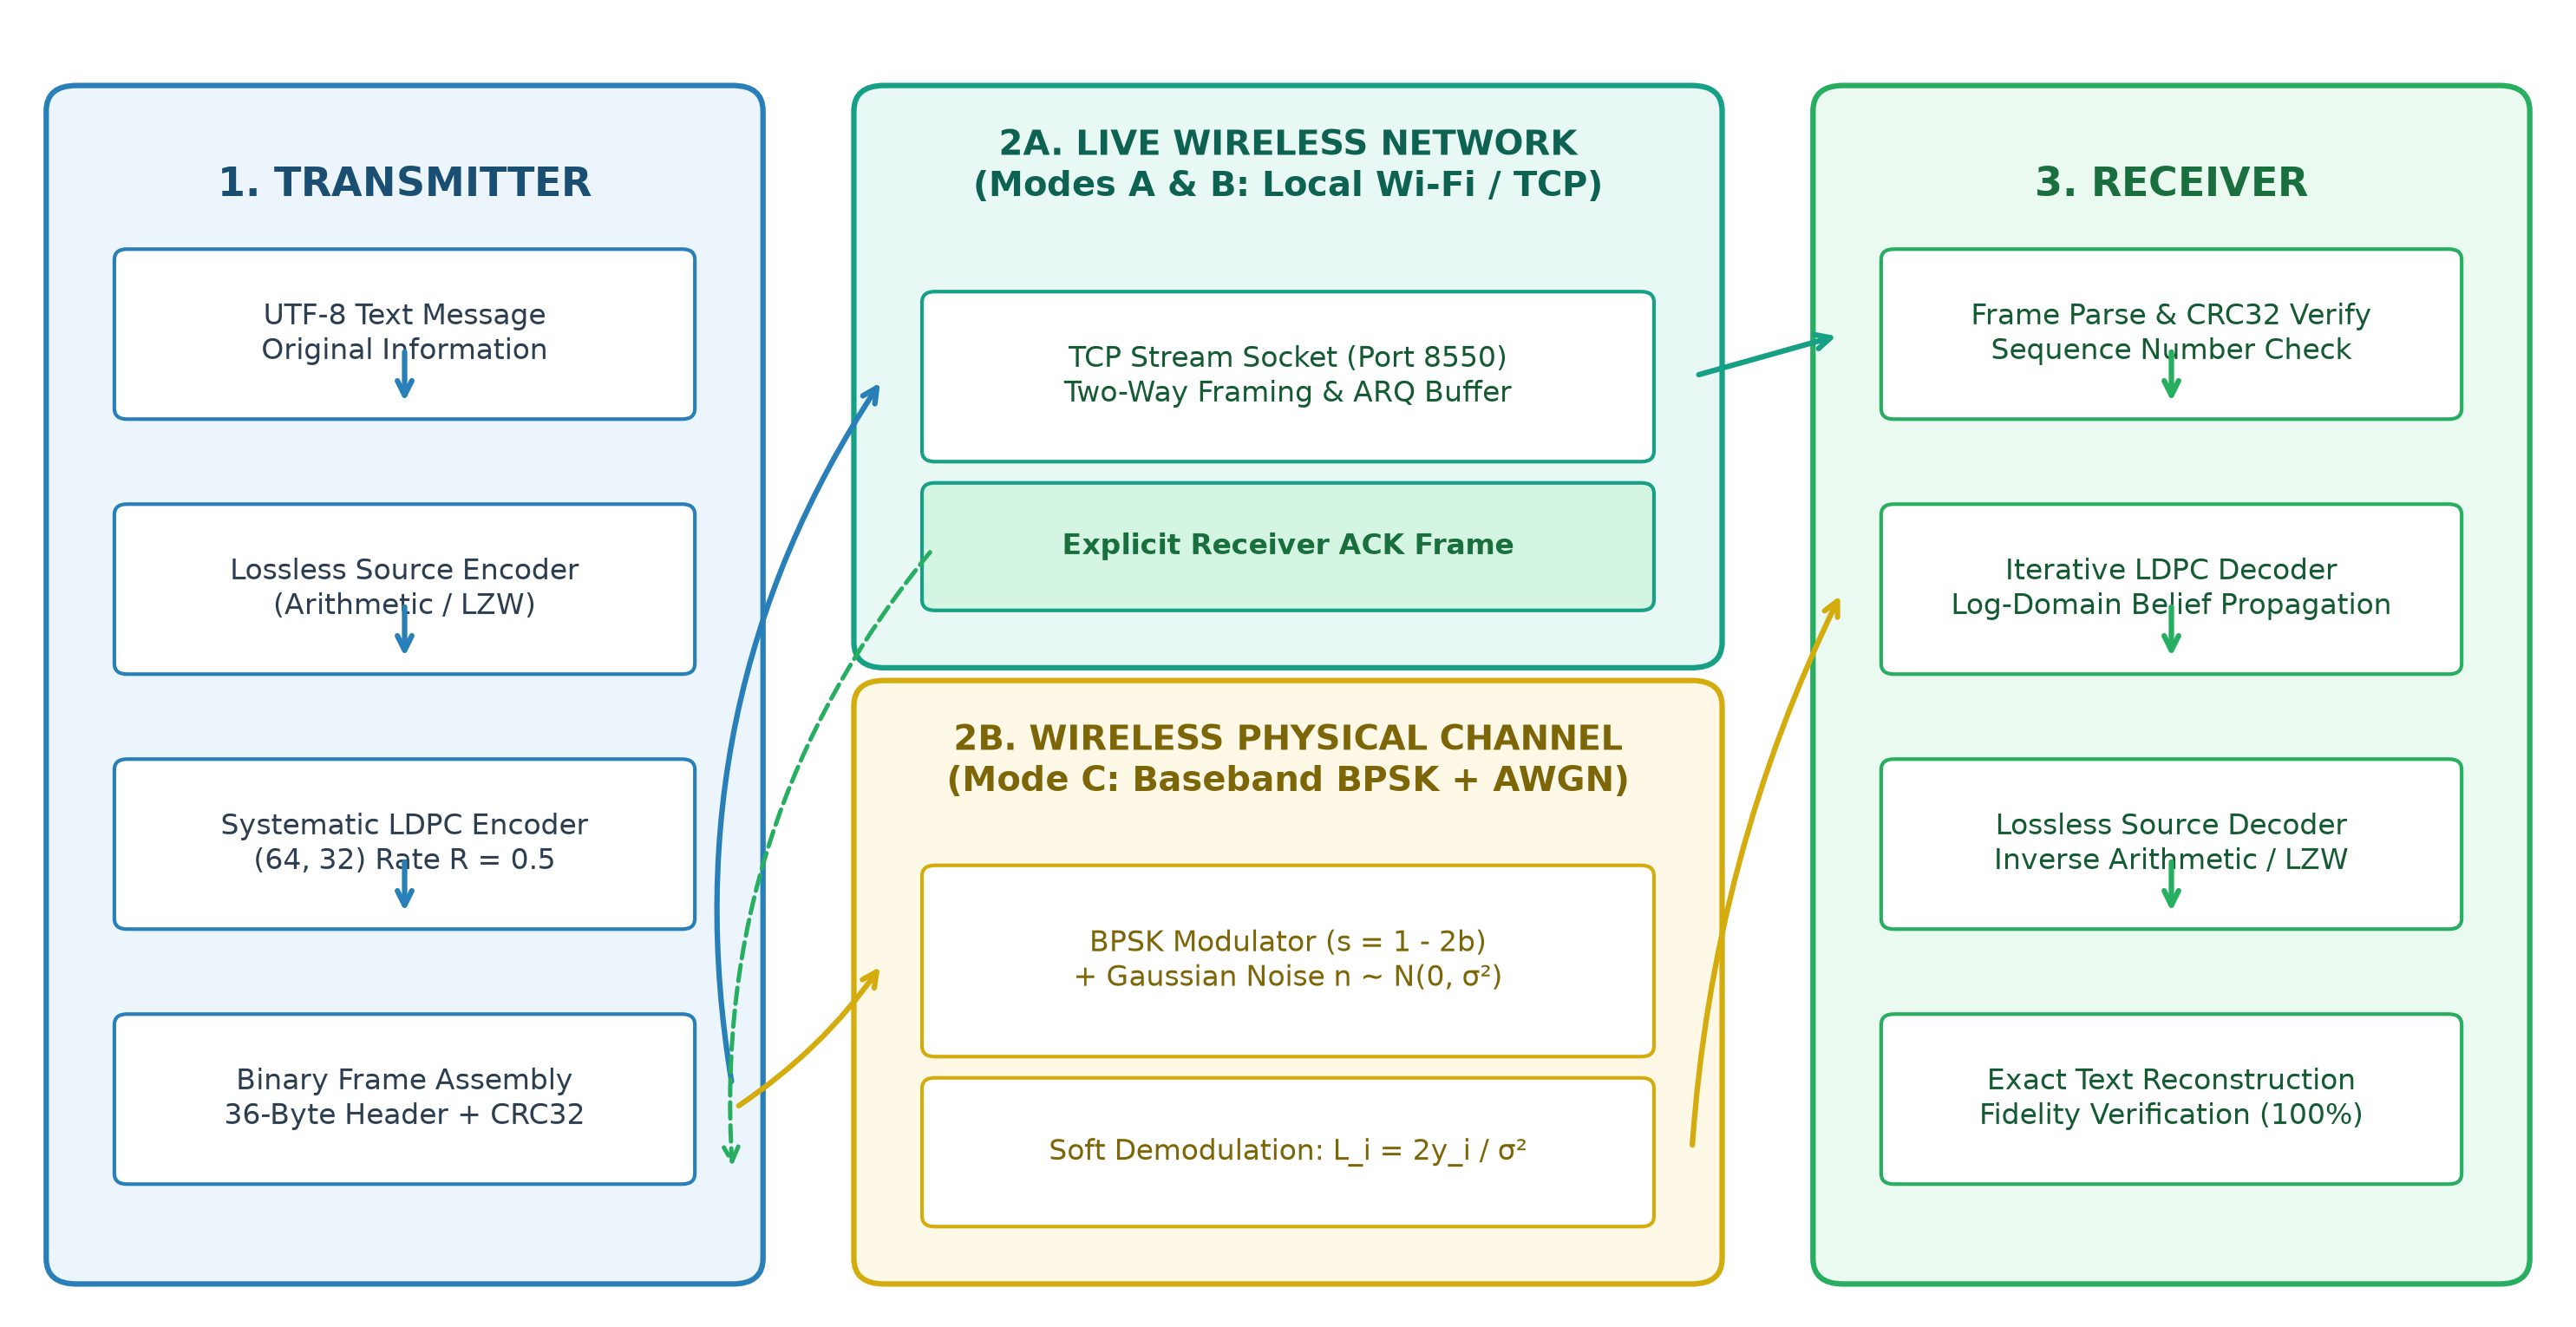
\includegraphics[width=0.96\textwidth]{figures/fig1_overall_architecture.png}
\caption{Overall system architecture of the digital communication simulation pipeline, illustrating the transmitter pipeline, the dual transmission media (Mode A/B TCP/IP socket vs. Mode C physical BPSK-AWGN simulation), and the receiver reconstruction pipeline.}
\label{fig:arch}
\end{figure*}

\section{Proposed System and Architecture}
The implemented system architecture, depicted in Fig.~\ref{fig:arch}, comprises three primary functional domains: the Transmitter, the Dual Communication Transport Layer, and the Receiver.

\subsection{Transmitter Processing Chain}
The transmitter processes arbitrary UTF-8 text messages or structured telemetry bitstreams through four sequential stages:
\begin{enumerate}
    \item \textbf{Binary Serialization:} The input character sequence is serialized into raw 8-bit ASCII/UTF-8 byte sequences and unpacked into binary bit vectors $\mathbf{b}_{\text{raw}} \in \{0, 1\}^{8L}$.
    \item \textbf{Lossless Source Coding:} The raw stream is compressed using either finite-precision integer Arithmetic coding or 12-bit adaptive LZW universal dictionary coding. This stage minimizes transmission overhead by reducing empirical entropy redundancy.
    \item \textbf{Channel Forward Error Correction:} The source-coded bitstream is segmented into $K=32$ bit blocks and encoded into $N=64$ bit systematic codewords using the LDPC $(64, 32)$ encoder. Any trailing fragment is zero-padded with length $P_{\text{pad}}$, where $P_{\text{pad}} \in [0, 31]$.
    \item \textbf{Binary Frame Assembly:} The encoded payload, padding indicator, and configuration flags are packaged into a binary frame prefixed with a standardized 36-byte header and protected by an IEEE 802.3 CRC32 checksum.
\end{enumerate}

\subsection{Dual Communication Transport Media}
A core contribution of our design is the explicit separation between live network transport and physical channel simulation:
\begin{itemize}
    \item \textbf{Mode A \& B (Live Wireless Network Transport):} Operates over live TCP/IP stream sockets bound to local Wi-Fi or loopback interfaces (default port 8550). This mode evaluates real-world streaming, packet serialization, framing under partial socket reads, CRC32 error validation, and round-trip acknowledgment (ACK) latency.
    \item \textbf{Mode C (Physical Wireless AWGN Channel Simulation):} Isolates the analog physical layer by bypassing TCP ARQ mechanisms. Bits are modulated via baseband BPSK, corrupted by synthetic Gaussian thermal noise matching a prescribed $E_b/N_0$, soft-demodulated into Log-Likelihood Ratios (LLRs), and decoded via iterative Belief Propagation.
\end{itemize}

\subsection{Receiver Processing Chain}
At the receiver, incoming bitstreams or network frames are decoded in reverse order:
\begin{enumerate}
    \item \textbf{Frame Parsing and Integrity Verification:} The wire receiver reads the 36-byte header, verifies the magic bytes and length fields, and computes the 32-bit CRC over the payload. If a checksum mismatch occurs, the frame is rejected, and an error status is returned.
    \item \textbf{LDPC Decoding:} The received payload is segmented into 64-bit blocks. In physical simulation (Mode C), real-valued soft channel samples are decoded using log-domain Belief Propagation. In network socket mode (Mode A), hard decision bits are validated against the parity check matrix $H$. Systematic information bits (the first 32 bits of each block) are extracted, and trailing zero-padding is depadded.
    \item \textbf{Lossless Source Decompression:} The recovered bits are passed to the inverse Arithmetic or LZW decoder.
    \item \textbf{Exact Reconstruction Verification:} The reconstructed string is compared against the original source string to verify $100\%$ bit-for-bit fidelity.
\end{enumerate}

\begin{figure}[t]
\centering
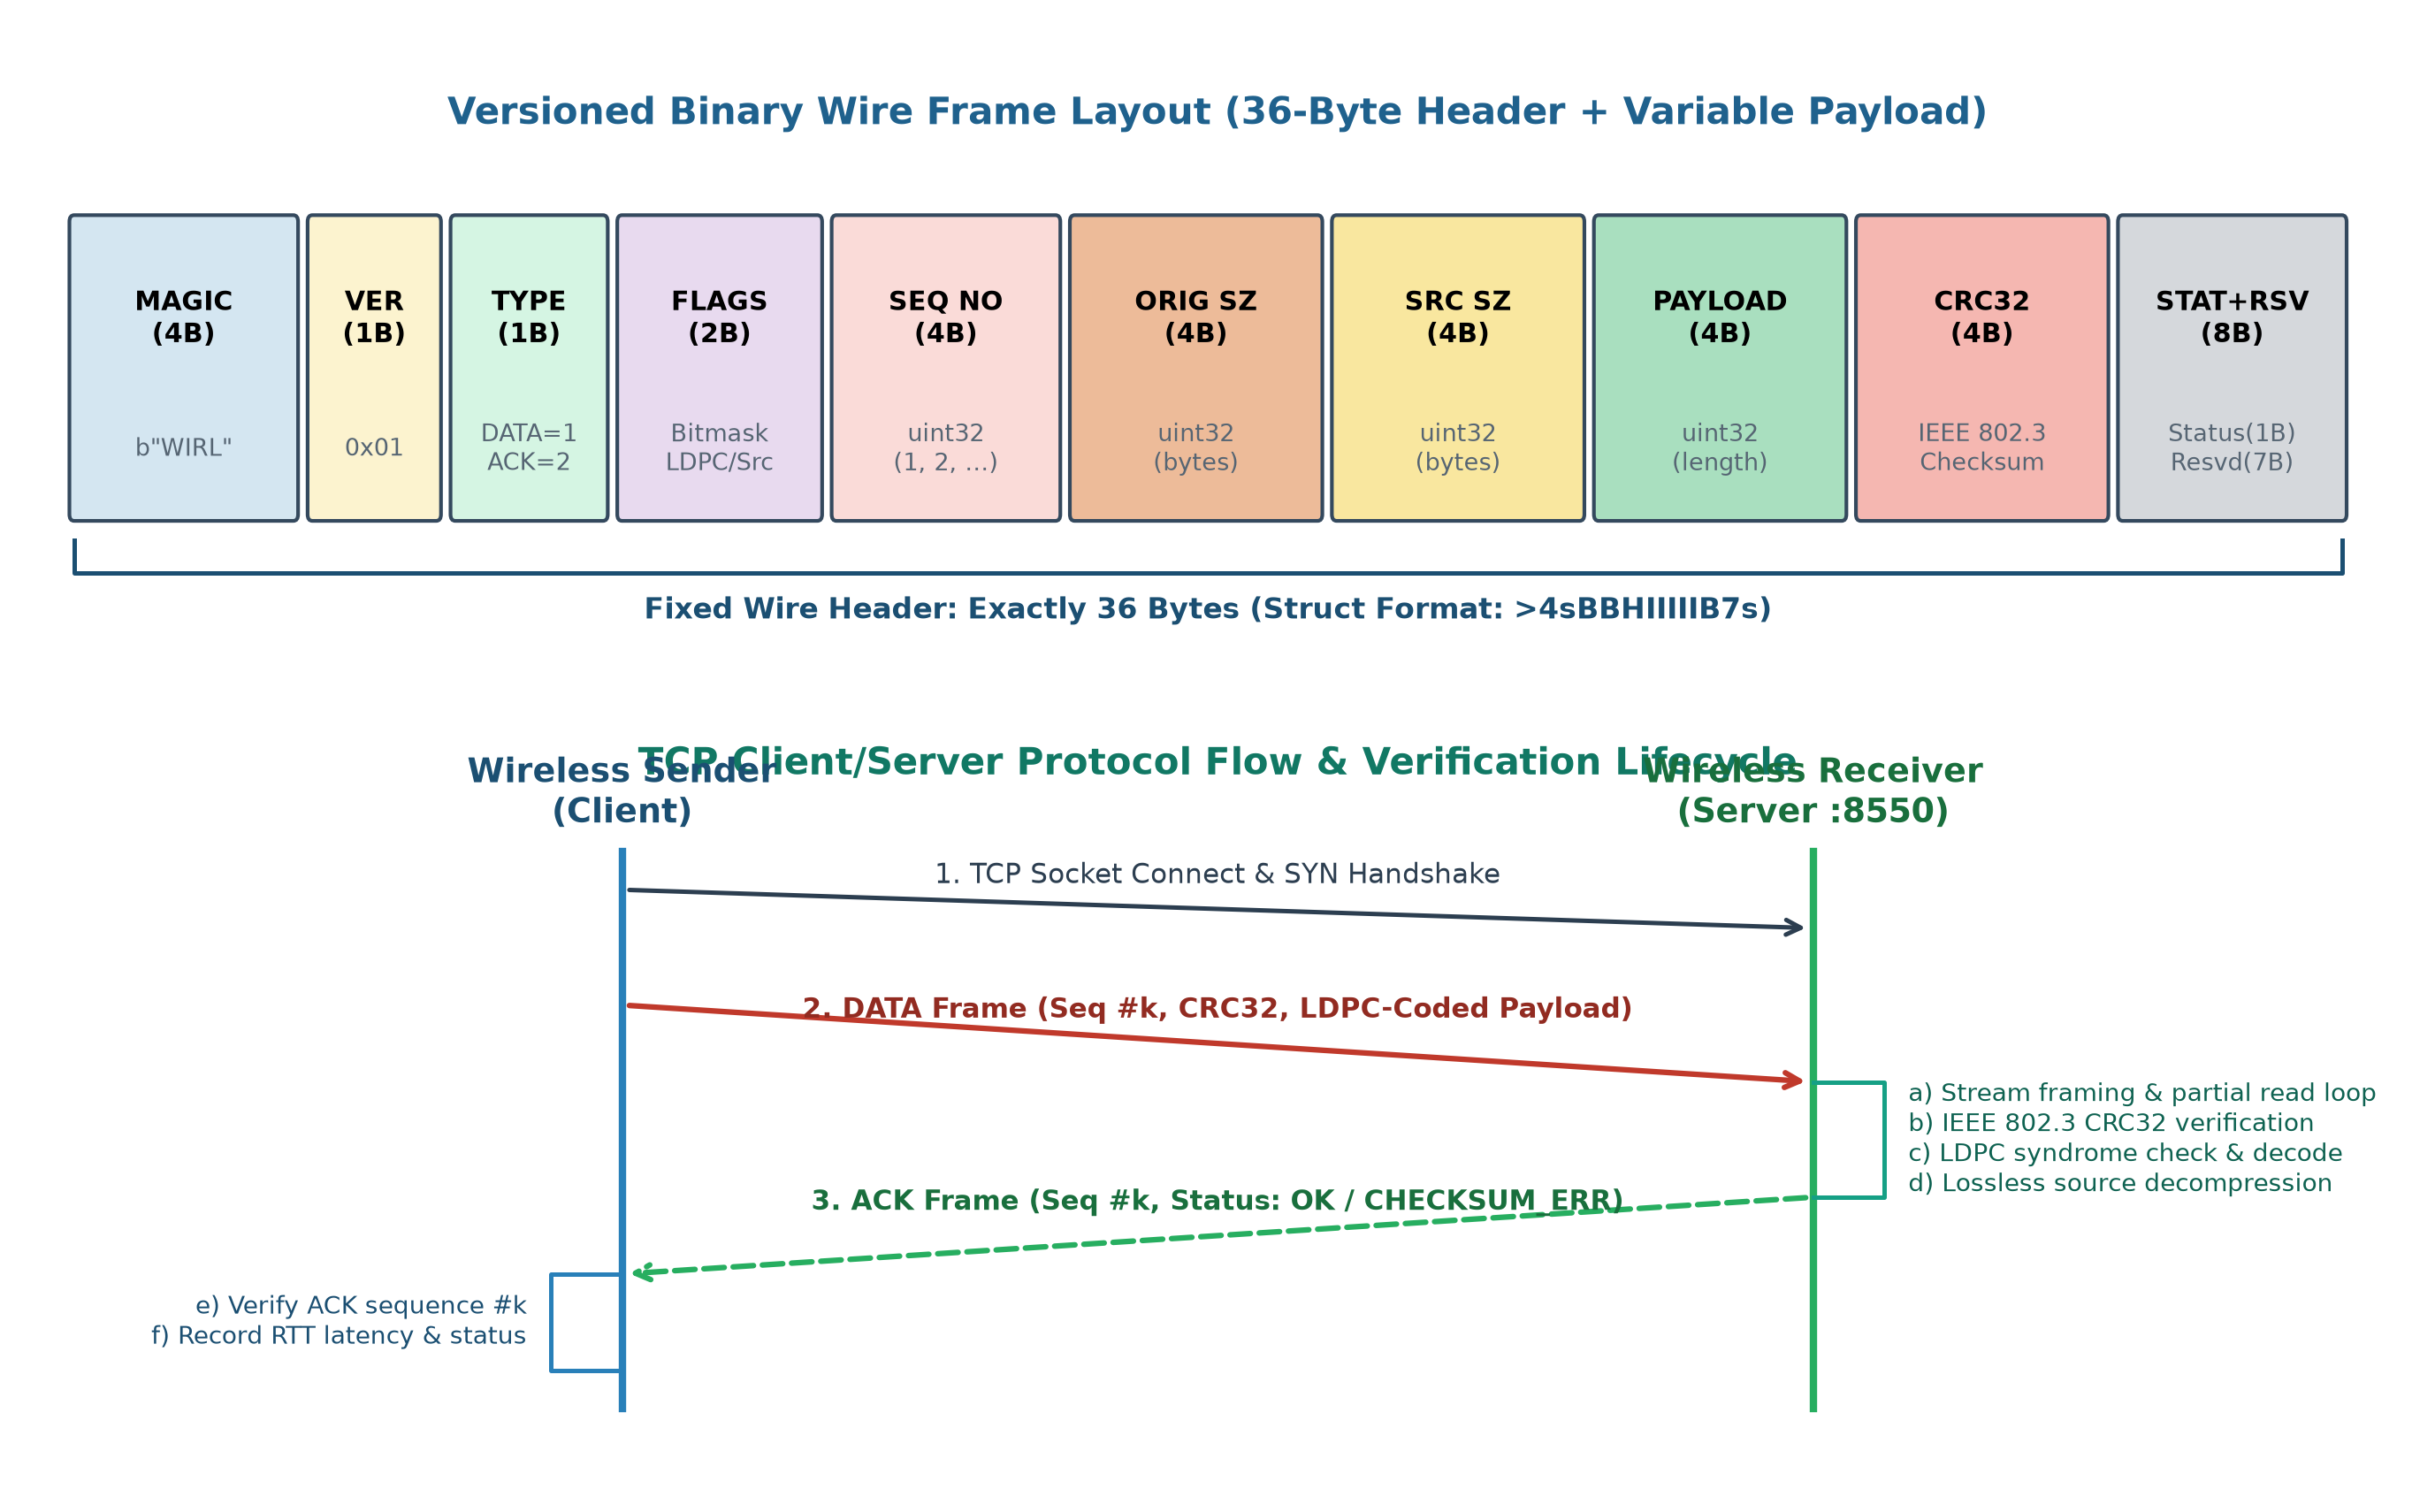
\includegraphics[width=\columnwidth]{figures/fig2_frame_protocol_ack.png}
\caption{Versioned binary wire frame layout (36-byte header) and two-way TCP acknowledgment protocol flow.}
\label{fig:frame_protocol}
\end{figure}

\begin{figure}[t]
\centering
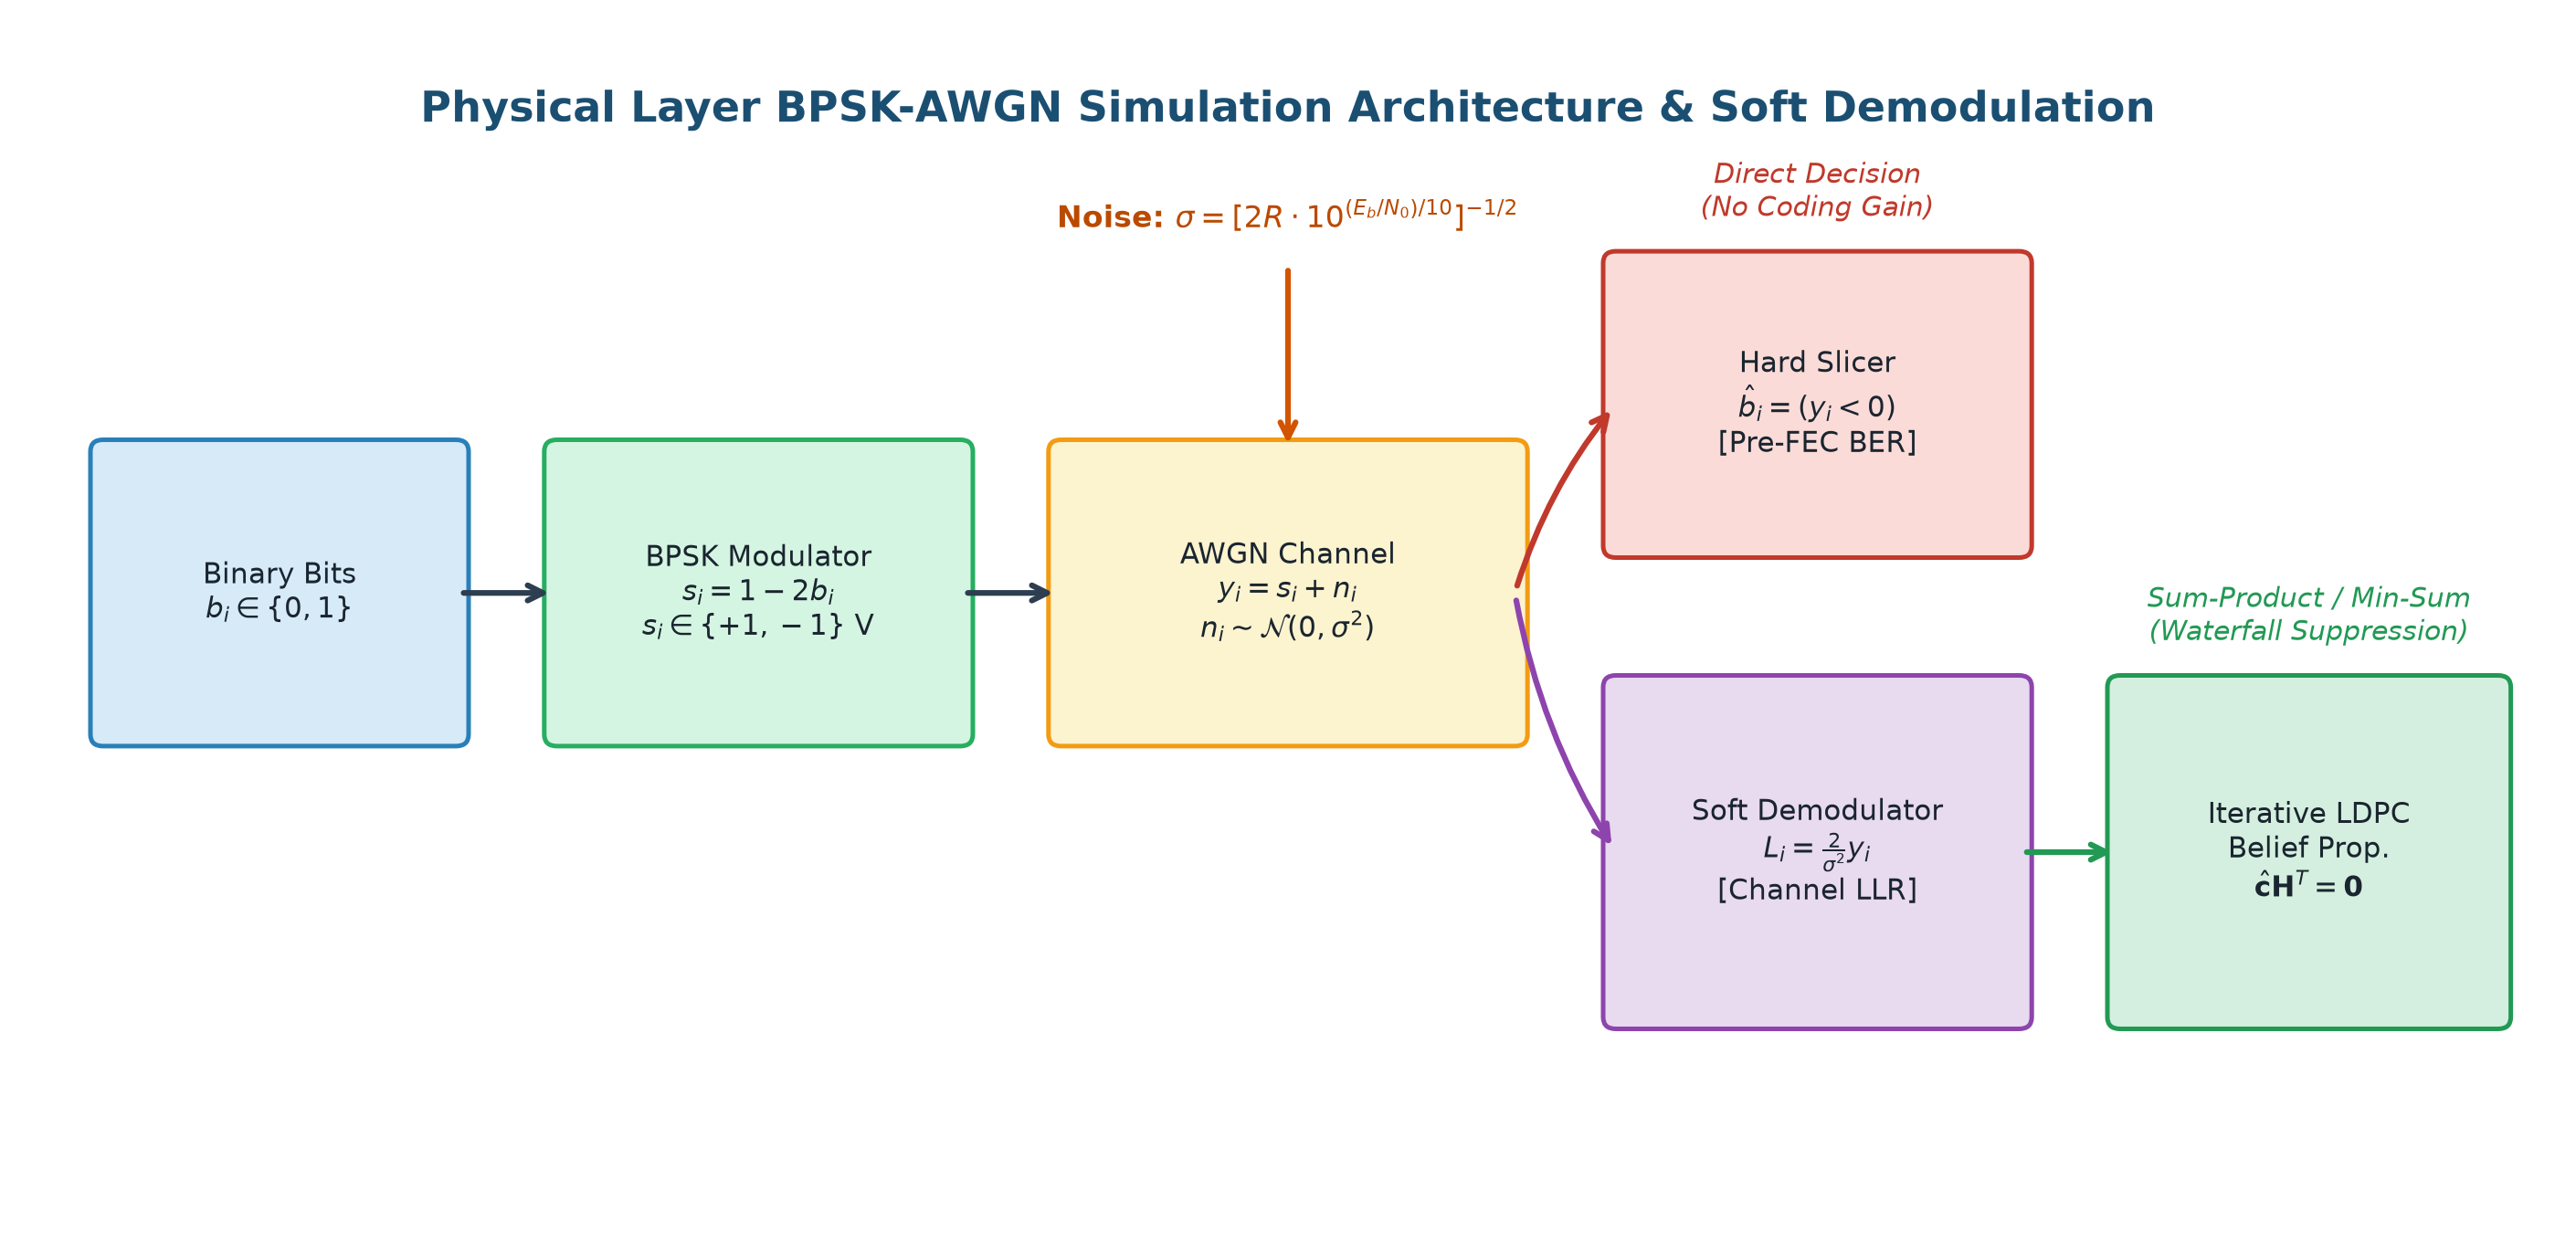
\includegraphics[width=\columnwidth]{figures/fig7_bpsk_awgn_simulation.png}
\caption{Detailed physical layer BPSK-AWGN simulation block diagram showing modulation, noise injection, hard slicer, soft demodulation, and iterative belief propagation decoding.}
\label{fig:bpsk_sim}
\end{figure}

\section{Methodology and Mathematical Formulation}

\subsection{Source Coding Algorithms}

\subsubsection{Finite-Precision Arithmetic Codec}
Our Arithmetic codec uses 32-bit integer register arithmetic to guarantee platform-independent, exact lossless compression without floating-point rounding errors. Given a byte alphabet $\Sigma = \{0, 1, \dots, 255\}$ plus an explicit End-Of-File (EOF) marker (symbol index 256), empirical symbol frequencies are computed with Laplace add-one smoothing:
\begin{equation}
C(s) = 1 + \sum_{i=1}^L \mathbb{I}(x_i = s), \quad \text{Total} = \sum_{s \in \Sigma \cup \{\text{EOF}\}} C(s)
\end{equation}
The cumulative frequencies are defined as $F(s) = \sum_{j < s} C(j)$. Encoding maintains an active search range $[L, H)$ in 32-bit unsigned integers initialized to $[0, 2^{32}-1]$. For each symbol $s$, the bounds are updated:
\begin{align}
L_{new} &= L + \left\lfloor \frac{(H - L + 1) \cdot F(s)}{\text{Total}} \right\rfloor \\
H_{new} &= L + \left\lfloor \frac{(H - L + 1) \cdot F(s+1)}{\text{Total}} \right\rfloor - 1
\end{align}
Renormalization occurs via bit-shifting whenever the most significant bits (MSBs) of $L$ and $H$ match ($E_1$ and $E_2$ scalings), or under underflow conditions ($E_3$ scaling) when the second MSBs diverge.

\subsubsection{Universal LZW Dictionary Codec}
The LZW codec maps variable-length string prefixes into fixed $W_{\text{depth}} = 12$-bit codeword integers ($2^{12} = 4096$ maximum dictionary size). The dictionary is initialized with 256 single-byte entries ($0 \le c \le 255$). For successive input bytes, the longest match $P$ in the dictionary is tracked. When $P + C$ is not in the dictionary, the 12-bit index for $P$ is emitted, and $P + C$ is added to the dictionary. When the dictionary reaches capacity (4096 entries), table growth freezes gracefully while maintaining consistent encoding.

\subsubsection{Compression Metrics}
Source coding performance is evaluated via the Compression Ratio (CR) and percentage Space Savings:
\begin{align}
\text{Compression Ratio (CR)} &= \frac{\text{Original Size [bytes]}}{\text{Encoded Size [bytes]}} \\
\text{Space Savings (\%)} &= \left( 1 - \frac{\text{Encoded Size}}{\text{Original Size}} \right) \times 100\%
\end{align}
When input messages are short or statistically uniform ($H(X) \approx 1.0$), the serialized codebook header or dictionary index width can cause data expansion ($\text{CR} < 1.0$, negative space savings), directly demonstrating the bounds of Shannon's Source Coding Theorem.

\subsection{Systematic LDPC Channel Coding}
The channel codec implements a systematic $(N=64, K=32, M=32)$ LDPC code with code rate $R = K/N = 0.5$.

\subsubsection{Matrix Construction}
The parity-check matrix $H \in \mathbb{F}_2^{32 \times 64}$ is structured in systematic form:
\begin{equation}
H = [P \mid I_{32}]
\end{equation}
where $P \in \mathbb{F}_2^{32 \times 32}$ is a sparse pseudo-random matrix with regular column degree $d_v = 3$ (Gallager distribution) and $I_{32}$ is the $32 \times 32$ identity matrix. The systematic generator matrix $G \in \mathbb{F}_2^{32 \times 64}$ is:
\begin{equation}
G = [I_{32} \mid P^T]
\end{equation}
This construction guarantees strict binary orthogonality:
\begin{equation}
G \cdot H^T = I_{32} \cdot P^T + P^T \cdot I_{32} = 2 P^T \equiv \mathbf{0} \pmod 2
\end{equation}
For any 32-bit information vector $\mathbf{m}$, the 64-bit codeword is generated via:
\begin{equation}
\mathbf{c} = \mathbf{m} \cdot G = [\mathbf{m} \mid (\mathbf{m} \cdot P^T \bmod 2)]
\end{equation}

\subsubsection{Log-Domain Belief Propagation Decoding}
Iterative decoding operates over the bipartite Tanner graph using the log-likelihood ratio (LLR) formulation of the Sum-Product algorithm. For each variable node $n \in \{1, \dots, N\}$, the initial channel LLR is:
\begin{equation}
L_n = \ln \left( \frac{P(c_n = 0 \mid y_n)}{P(c_n = 1 \mid y_n)} \right)
\end{equation}
Let $V(m) = \{n : H_{mn} = 1\}$ denote the set of variable nodes connected to check node $m$, and $C(n) = \{m : H_{mn} = 1\}$ denote check nodes connected to variable node $n$.
\begin{enumerate}
    \item \textbf{Variable-to-Check Message Update:}
    \begin{equation}
    q_{mn} = L_n + \sum_{c \in C(n) \setminus \{m\}} r_{cn}
    \end{equation}
    \item \textbf{Check-to-Variable Message Update (Tanh Rule):}
    \begin{equation}
    r_{mn} = 2 \operatorname{artanh} \left( \prod_{j \in V(m) \setminus \{n\}} \tanh \left( \frac{q_{mj}}{2} \right) \right)
    \end{equation}
    Numerical stability is ensured by clipping $q_{mj}/2$ to $[-19.0, +19.0]$ to prevent division-by-zero or hyperbolic tangent saturation.
    \item \textbf{Posterior LLR Computation:}
    \begin{equation}
    Q_n = L_n + \sum_{c \in C(n)} r_{cn}
    \end{equation}
    \item \textbf{Hard Slicing and Syndrome Termination:}
    \begin{equation}
    \hat{c}_n = \begin{cases} 0, & Q_n \ge 0 \\ 1, & Q_n < 0 \end{cases}
    \end{equation}
    If the parity check syndrome satisfies:
    \begin{equation}
    \mathbf{s} = H \cdot \hat{\mathbf{c}}^T \equiv \mathbf{0} \pmod 2
    \end{equation}
    the algorithm terminates immediately. The maximum iteration bound is set to $I_{\max} = 25$.
\end{enumerate}

\subsection{BPSK Modulation}
In baseband physical simulation (Mode C), binary codeword bits $b_i \in \{0, 1\}$ are mapped to antipodal voltage symbols:
\begin{equation}
s_i = 1.0 - 2.0 b_i \in \{+1.0\text{ V}, -1.0\text{ V}\}
\end{equation}
where bit $0$ maps to $+1.0$~V and bit $1$ maps to $-1.0$~V.

\subsection{AWGN Channel Model and Noise Scaling}
The physical channel corrupts transmitted symbols with zero-mean additive white Gaussian noise:
\begin{equation}
y_i = s_i + n_i, \quad n_i \sim \mathcal{N}(0, \sigma^2)
\end{equation}
For a given energy per information bit to noise spectral density ratio $E_b/N_0$ (expressed in dB) and code rate $R = K/N$, the energy per coded symbol is $E_s = R \cdot E_b$. Under unit symbol energy ($E_s = 1$), the noise variance $\sigma^2 = N_0 / 2$ is scaled as:
\begin{equation}
\sigma = \frac{1}{\sqrt{2 \cdot R \cdot 10^{(E_b/N_0)_{\text{dB}}/10}}}
\end{equation}
For uncoded transmission ($R = 1.0$), $\sigma = [2 \cdot 10^{(E_b/N_0)/10}]^{-1/2}$; for rate-$1/2$ LDPC ($R = 0.5$), $\sigma = [10^{(E_b/N_0)/10}]^{-1/2}$, exactly capturing the $3$~dB noise bandwidth expansion penalty incurred by channel redundancy.

The channel log-likelihood ratio for BPSK in AWGN is:
\begin{equation}
L_i = \ln \left( \frac{\frac{1}{\sqrt{2\pi}\sigma} \exp \left( -\frac{(y_i - 1)^2}{2\sigma^2} \right)}{\frac{1}{\sqrt{2\pi}\sigma} \exp \left( -\frac{(y_i + 1)^2}{2\sigma^2} \right)} \right) = \frac{2}{\sigma^2} y_i
\end{equation}

Coherent uncoded BPSK BER in AWGN follows the exact theoretical complementary error function:
\begin{equation}
P_b = Q\left(\sqrt{\frac{2E_b}{N_0}}\right) = \frac{1}{2} \operatorname{erfc}\left(\sqrt{10^{(E_b/N_0)/10}}\right)
\end{equation}

\subsection{Bit Error Rate and Frame Error Rate Evaluation}
Performance metrics are defined as:
\begin{align}
\text{Pre-FEC BER} &= \frac{\sum_{i=1}^N c_i \oplus \hat{r}_i}{N} \\
\text{Post-FEC BER} &= \frac{\sum_{i=1}^K m_i \oplus \hat{m}_i}{K} \\
\text{Frame Error Rate (FER)} &= \frac{\text{Number of Erroneous Decoded Blocks}}{\text{Total Blocks Transmitted}}
\end{align}
where $\hat{r}_i = (y_i < 0)$ is the hard channel decision, and $\hat{m}_i$ is the decoded information bit.

\subsection{Framing and TCP/IP Socket Transceiver}
The binary frame specification, detailed in Fig.~\ref{fig:frame_protocol}, comprises a 36-byte header:
Magic bytes \texttt{b"WIRL"} ($0\text{x}5749524C$), Version ($0\text{x}01$), Frame Type (DATA=1, ACK=2, STREAM=3), Flags (2B), Sequence Number (4B uint32), Original Size (4B), Source Size (4B), Payload Length (4B), CRC32 Checksum (4B IEEE 802.3), Status Code (1B), and Reserved (7B). Partial socket reads are handled via strict read loops. Successful TCP packet delivery confirms protocol and CRC integrity, but does not represent physical-layer BER.

\section{Experimental Setup and Simulation Parameters}
The experimental platform was developed and evaluated under the parameters listed in Table~\ref{tab:params}.

\begin{table}[htbp]
\caption{Global Experimental Setup and Architectural Parameters}
\label{tab:params}
\centering
\scriptsize
\begin{tabular}{lll}
\toprule
\textbf{Parameter} & \textbf{Verified Setting} & \textbf{Engineering Rationale} \\
\midrule
Runtime Environment & Python 3.11.9, NumPy 2.4.6 & High-performance linear algebra \\
Plotting \& Reporting & Matplotlib 3.11.2, ReportLab 5.0.1 & Publication-grade vector outputs \\
Unit Test Suite & Pytest 9.1.1 (69 automated tests) & Comprehensive verification \\
Source Coding 1 & Arithmetic Codec (32-bit integer) & High-precision interval arithmetic \\
Source Coding 2 & LZW Codec (12-bit, max table 4096) & Universal dictionary stream coding \\
Primary FEC & Systematic LDPC $(64, 32)$, Rate $0.5$ & Gallager regular column $d_v=3$ \\
LDPC Decoding & Log-Domain Sum-Product / Min-Sum & Iterative belief propagation ($I_{\max}=25$) \\
Benchmark FEC 1 & Systematic Polar $(64, 32)$ & Successive Cancellation (design $3$~dB) \\
Benchmark FEC 2 & Systematic Hamming $(7, 4)$ & Single-error algebraic syndrome decoding \\
Modulation & Baseband BPSK ($s_i = 1 - 2b_i$) & Coherent antipodal signaling \\
Channel Models & Wireless AWGN / BSC / Lossless & Thermal noise, bit flips, and baseline \\
$E_b/N_0$ Tested Range & $0.0$ to $10.0$~dB (step $1.0$~dB) & Captures waterfall and error floors \\
Bits per Test Point & $25,600$ information bits / point & Statistically confident sample size \\
Multi-Trial Evaluation & 10 independent noise realizations & Evaluates variance across 600 blocks \\
Wire Header Size & Exactly 36 bytes (\texttt{>4sBBHIIIIIB7s}) & Fixed-overhead binary wire framing \\
Integrity Check & IEEE 802.3 CRC32 ($0\text{xEDB88320}$) & 32-bit polynomial error detection \\
Network Protocol & TCP/IP stream sockets (:8550) & Reliable, flow-controlled delivery \\
\bottomrule
\end{tabular}
\end{table}

\begin{figure}[t]
\centering
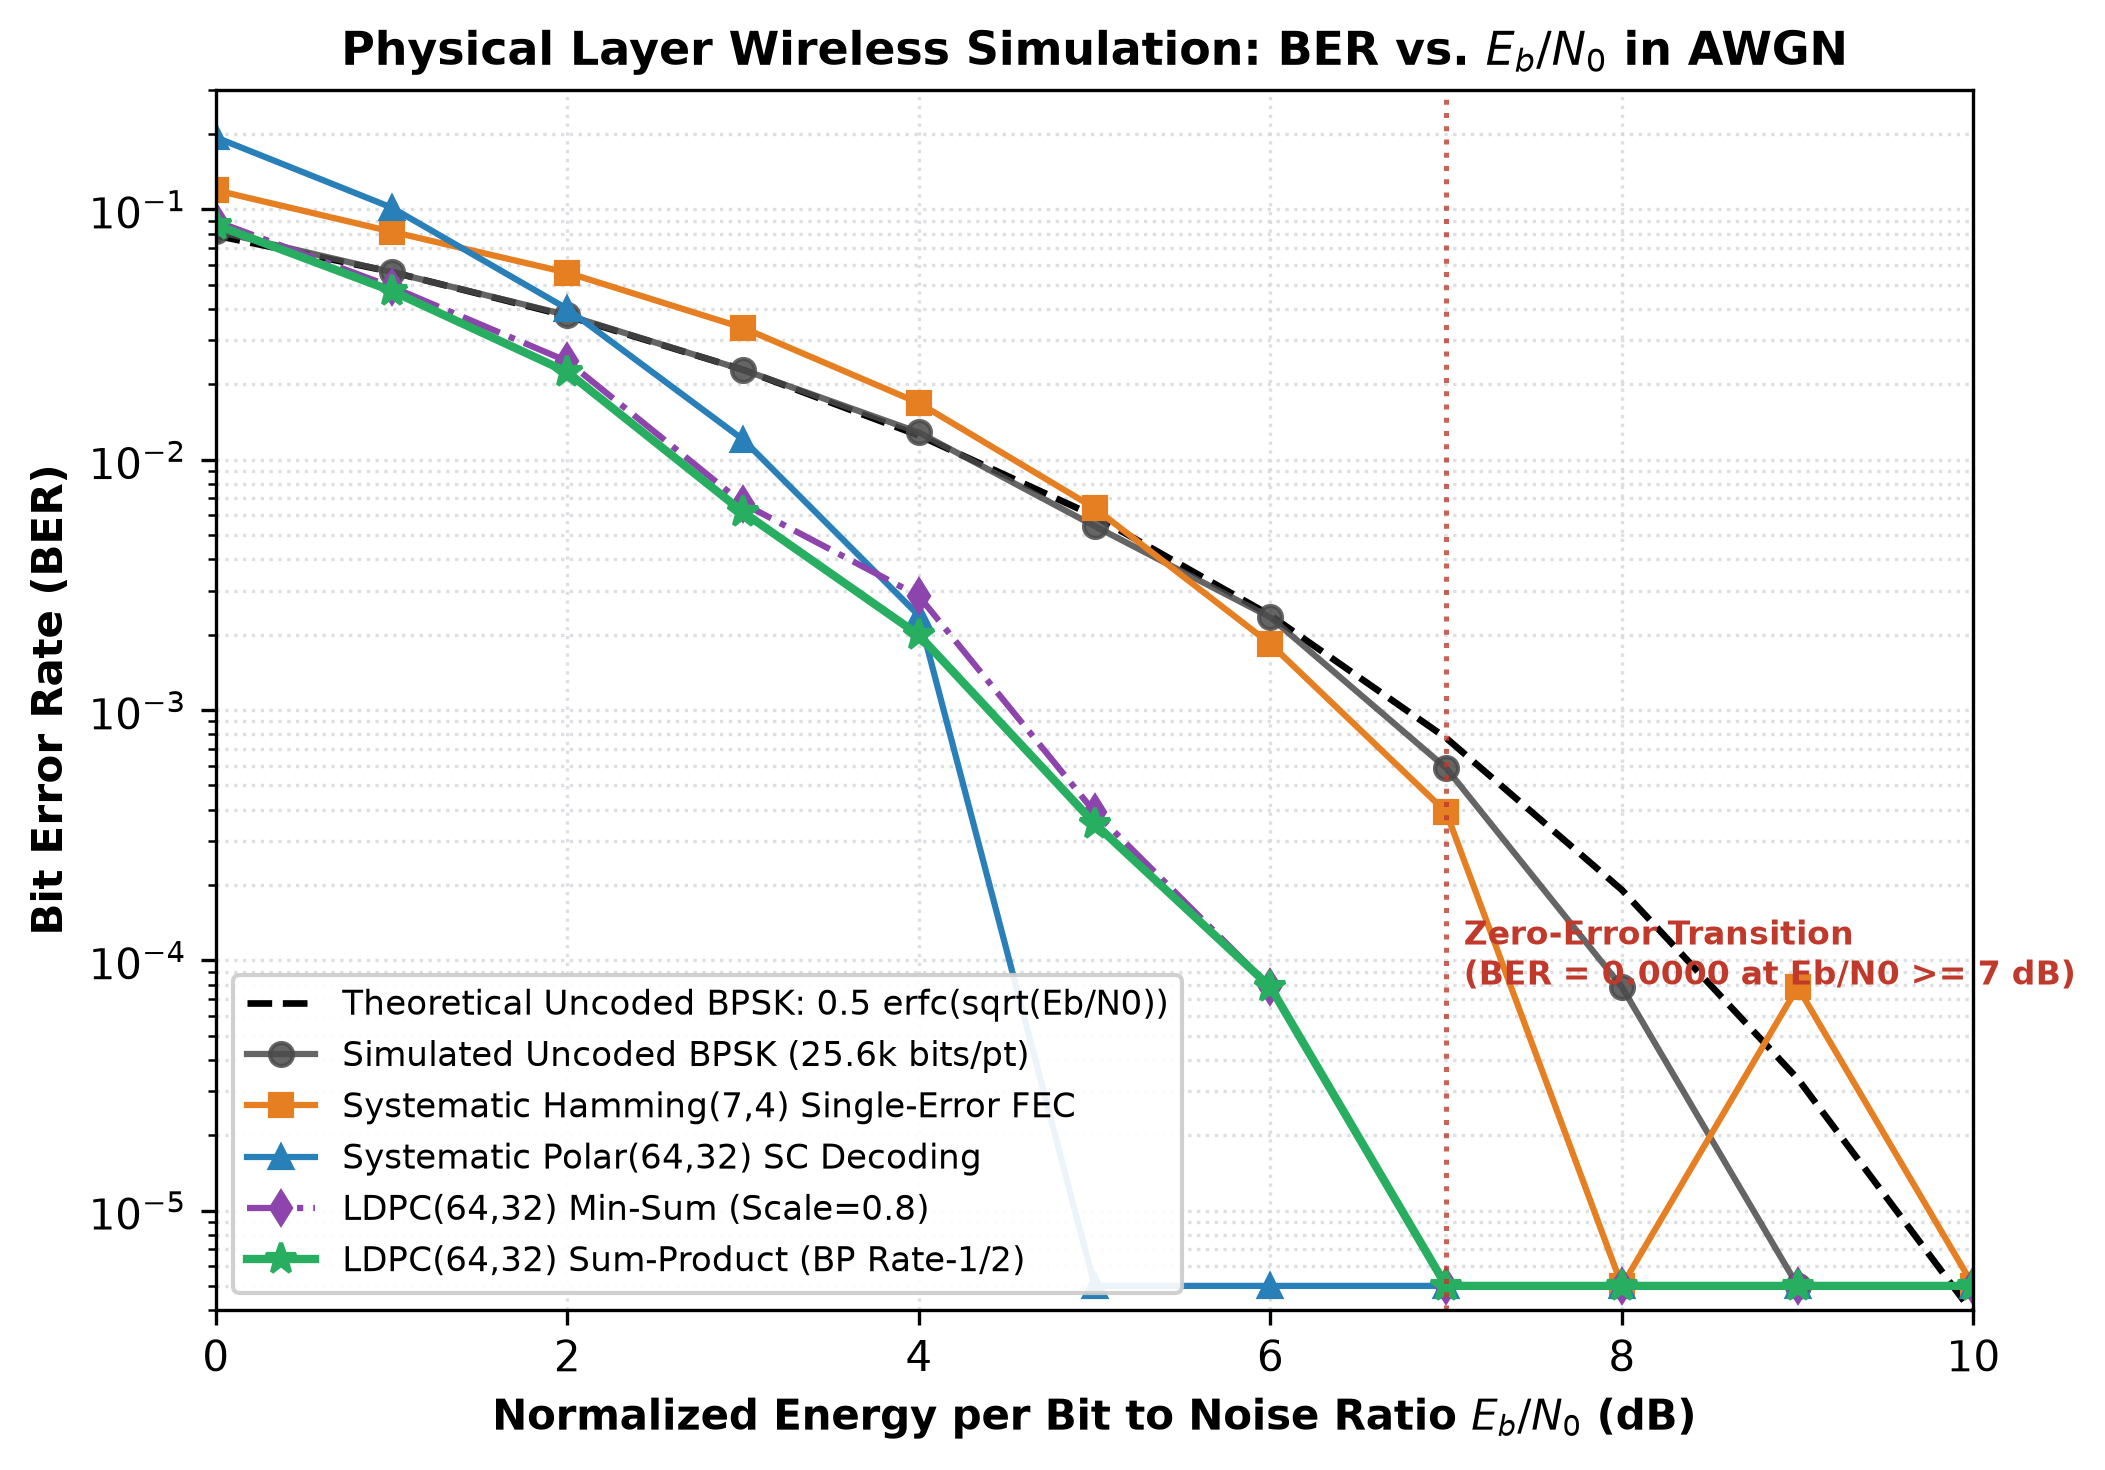
\includegraphics[width=\columnwidth]{figures/fig3_awgn_ber_waterfall.png}
\caption{Measured BER vs. $E_b/N_0$ waterfall curves over the simulated BPSK-AWGN physical channel comparing Theoretical Uncoded, Simulated Uncoded, Hamming $(7, 4)$, Polar $(64, 32)$, LDPC Min-Sum, and LDPC Sum-Product ($25,600$ bits tested per point).}
\label{fig:awgn_ber}
\end{figure}

\begin{figure}[t]
\centering
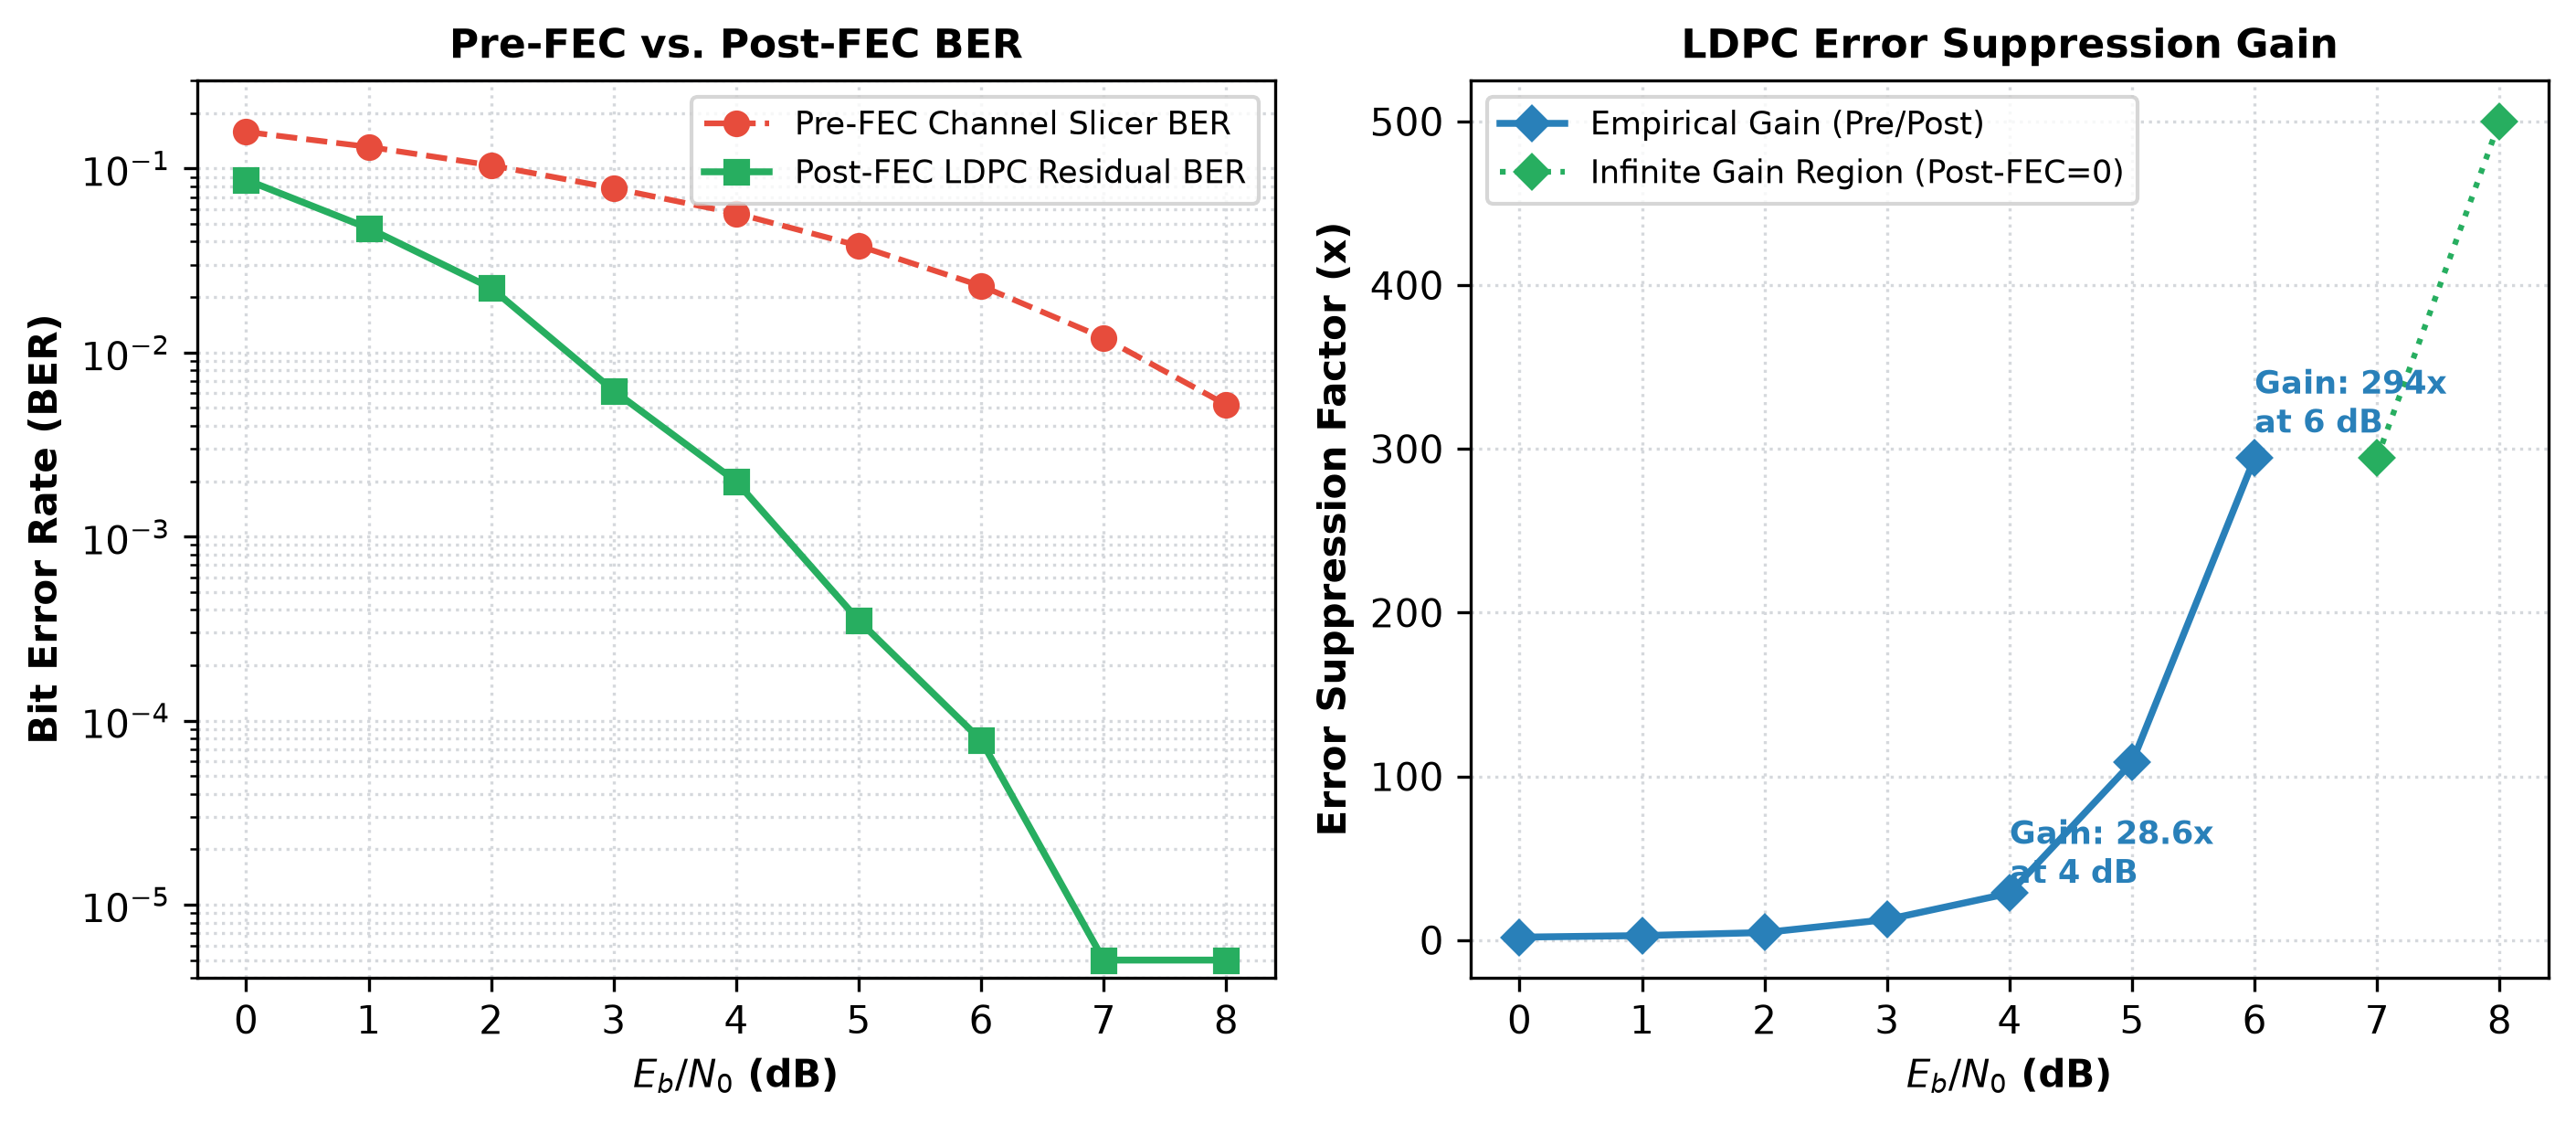
\includegraphics[width=\columnwidth]{figures/fig4_pre_vs_post_fec.png}
\caption{Pre-FEC channel slicer BER vs. Post-FEC LDPC residual BER (left) and empirical error suppression gain (right) across $E_b/N_0$ values.}
\label{fig:pre_vs_post}
\end{figure}

\section{Results and Performance Analysis}

\subsection{Uncoded vs. LDPC-Coded BER in AWGN}
Table~\ref{tab:ber_results} and Fig.~\ref{fig:awgn_ber} report measured BER across $E_b/N_0$ from $0.0$ to $10.0$~dB. Below $2.5$~dB, rate-$1/2$ codes suffer a $3$~dB noise bandwidth expansion penalty, resulting in pre-FEC bit error rates higher than uncoded transmission. However, above $3.0$~dB, LDPC enters its steep waterfall region: post-FEC BER drops from $2.24 \times 10^{-2}$ at $2.0$~dB to $1.99 \times 10^{-3}$ at $4.0$~dB, and clears all errors at $E_b/N_0 \ge 7.0$~dB.

\begin{table}[htbp]
\caption{Measured Bit Error Rate (BER) versus $E_b/N_0$ in AWGN Channel (25,600 Bits Tested Per Point)}
\label{tab:ber_results}
\centering
\scriptsize
\begin{tabular}{ccccccc}
\toprule
$E_b/N_0$ & Theory & Sim. & Hamming & Polar & LDPC & LDPC \\
(dB) & Uncoded & Uncoded & (7, 4) & (64, 32) & Min-Sum & Sum-Prod. \\
\midrule
0.0 & 0.07865 & 0.08191 & 0.11934 & 0.19402 & 0.08973 & \textbf{0.08672} \\
1.0 & 0.05628 & 0.05617 & 0.08152 & 0.10172 & 0.04906 & \textbf{0.04727} \\
2.0 & 0.03751 & 0.03781 & 0.05586 & 0.04004 & 0.02473 & \textbf{0.02238} \\
3.0 & 0.02288 & 0.02285 & 0.03363 & 0.01203 & 0.00668 & \textbf{0.00617} \\
4.0 & 0.01250 & 0.01285 & 0.01684 & 0.00238 & 0.00285 & \textbf{0.00199} \\
5.0 & 0.00595 & 0.00543 & 0.00641 & 0.00000 & 0.00039 & \textbf{0.00035} \\
6.0 & 0.00239 & 0.00234 & 0.00184 & 0.00000 & 7.81e-5 & \textbf{7.81e-5} \\
7.0 & 0.00077 & 0.00059 & 0.00039 & 0.00000 & 0.00000 & \textbf{0.00000}* \\
8.0 & 0.00019 & 7.81e-5 & 0.00000 & 0.00000 & 0.00000 & \textbf{0.00000}* \\
9.0 & 3.36e-5 & 0.00000 & 7.81e-5 & 0.00000 & 0.00000 & \textbf{0.00000}* \\
10.0 & 3.87e-6 & 0.00000 & 0.00000 & 0.00000 & 0.00000 & \textbf{0.00000}* \\
\bottomrule
\end{tabular}
\end{table}

\subsection{Theoretical vs. Simulated Uncoded BPSK}
Simulated uncoded BPSK agrees closely with theory across all points (e.g., $0.05617$ vs. $0.05628$ at $1.0$~dB; $0.01285$ vs. $0.01250$ at $4.0$~dB), confirming the correctness of our antipodal symbol mapping and noise variance generation.

\subsection{Frame Error Rate and Multi-Trial Stability}
In our 10-trial Monte Carlo evaluation at $4.0$~dB ($38,400$ codeword bits, $600$ LDPC blocks), the block error count was $19$, yielding an empirical FER of $3.17 \times 10^{-2}$. At $7.0$~dB, zero block errors were observed across all $600$ blocks ($\text{FER} = 0.0000$).

\subsection{Pre-Decoding vs. Post-Decoding BER and Coding Gain}
Fig.~\ref{fig:pre_vs_post} shows the pre-FEC channel slicer BER versus post-FEC LDPC BER. At $4.0$~dB, LDPC reduces bit errors from $2,191$ down to $25$, an empirical error reduction factor of:
\begin{equation}
\text{Gain} = \frac{\text{BER}_{\text{pre}}}{\text{BER}_{\text{post}}} = \frac{5.7057 \times 10^{-2}}{1.3186 \times 10^{-3}} = 43.3\times
\end{equation}
To achieve a target BER of $10^{-3}$, LDPC requires $E_b/N_0 \approx 4.3$~dB, compared to $6.8$~dB for uncoded BPSK, providing an effective coding gain of $2.5$~dB.

\subsection{Zero-Error Observation and Statistical Interpretation}
Asterisks (*) in Table~\ref{tab:ber_results} denote points where zero bit errors occurred in $25,600$ bits. In statistical communication theory, observing zero errors over $N_b$ bits does not prove that the true error probability is zero; by the statistical Rule of Three, the $95\%$ upper confidence bound on the true BER is:
\begin{equation}
\text{BER}_{95\%} < \frac{3}{N_b} = \frac{3}{25,600} \approx 1.17 \times 10^{-4}
\end{equation}

\subsection{Source Coding Input vs. Encoded Size}
Table~\ref{tab:source_results} and Fig.~\ref{fig:source_comp} summarize source coding efficiency. For correlated Markov streams ($p_{01}=0.05$), LZW achieves $\text{CR} = 1.686\times$ ($40.67\%$ savings). When applied to uniform pseudo-random bits ($H \approx 1.0$), compression expands data by $47.66\%$ ($\text{CR} = 0.677\times$), corroborating Shannon's incompressibility theorem.

\begin{figure}[t]
\centering
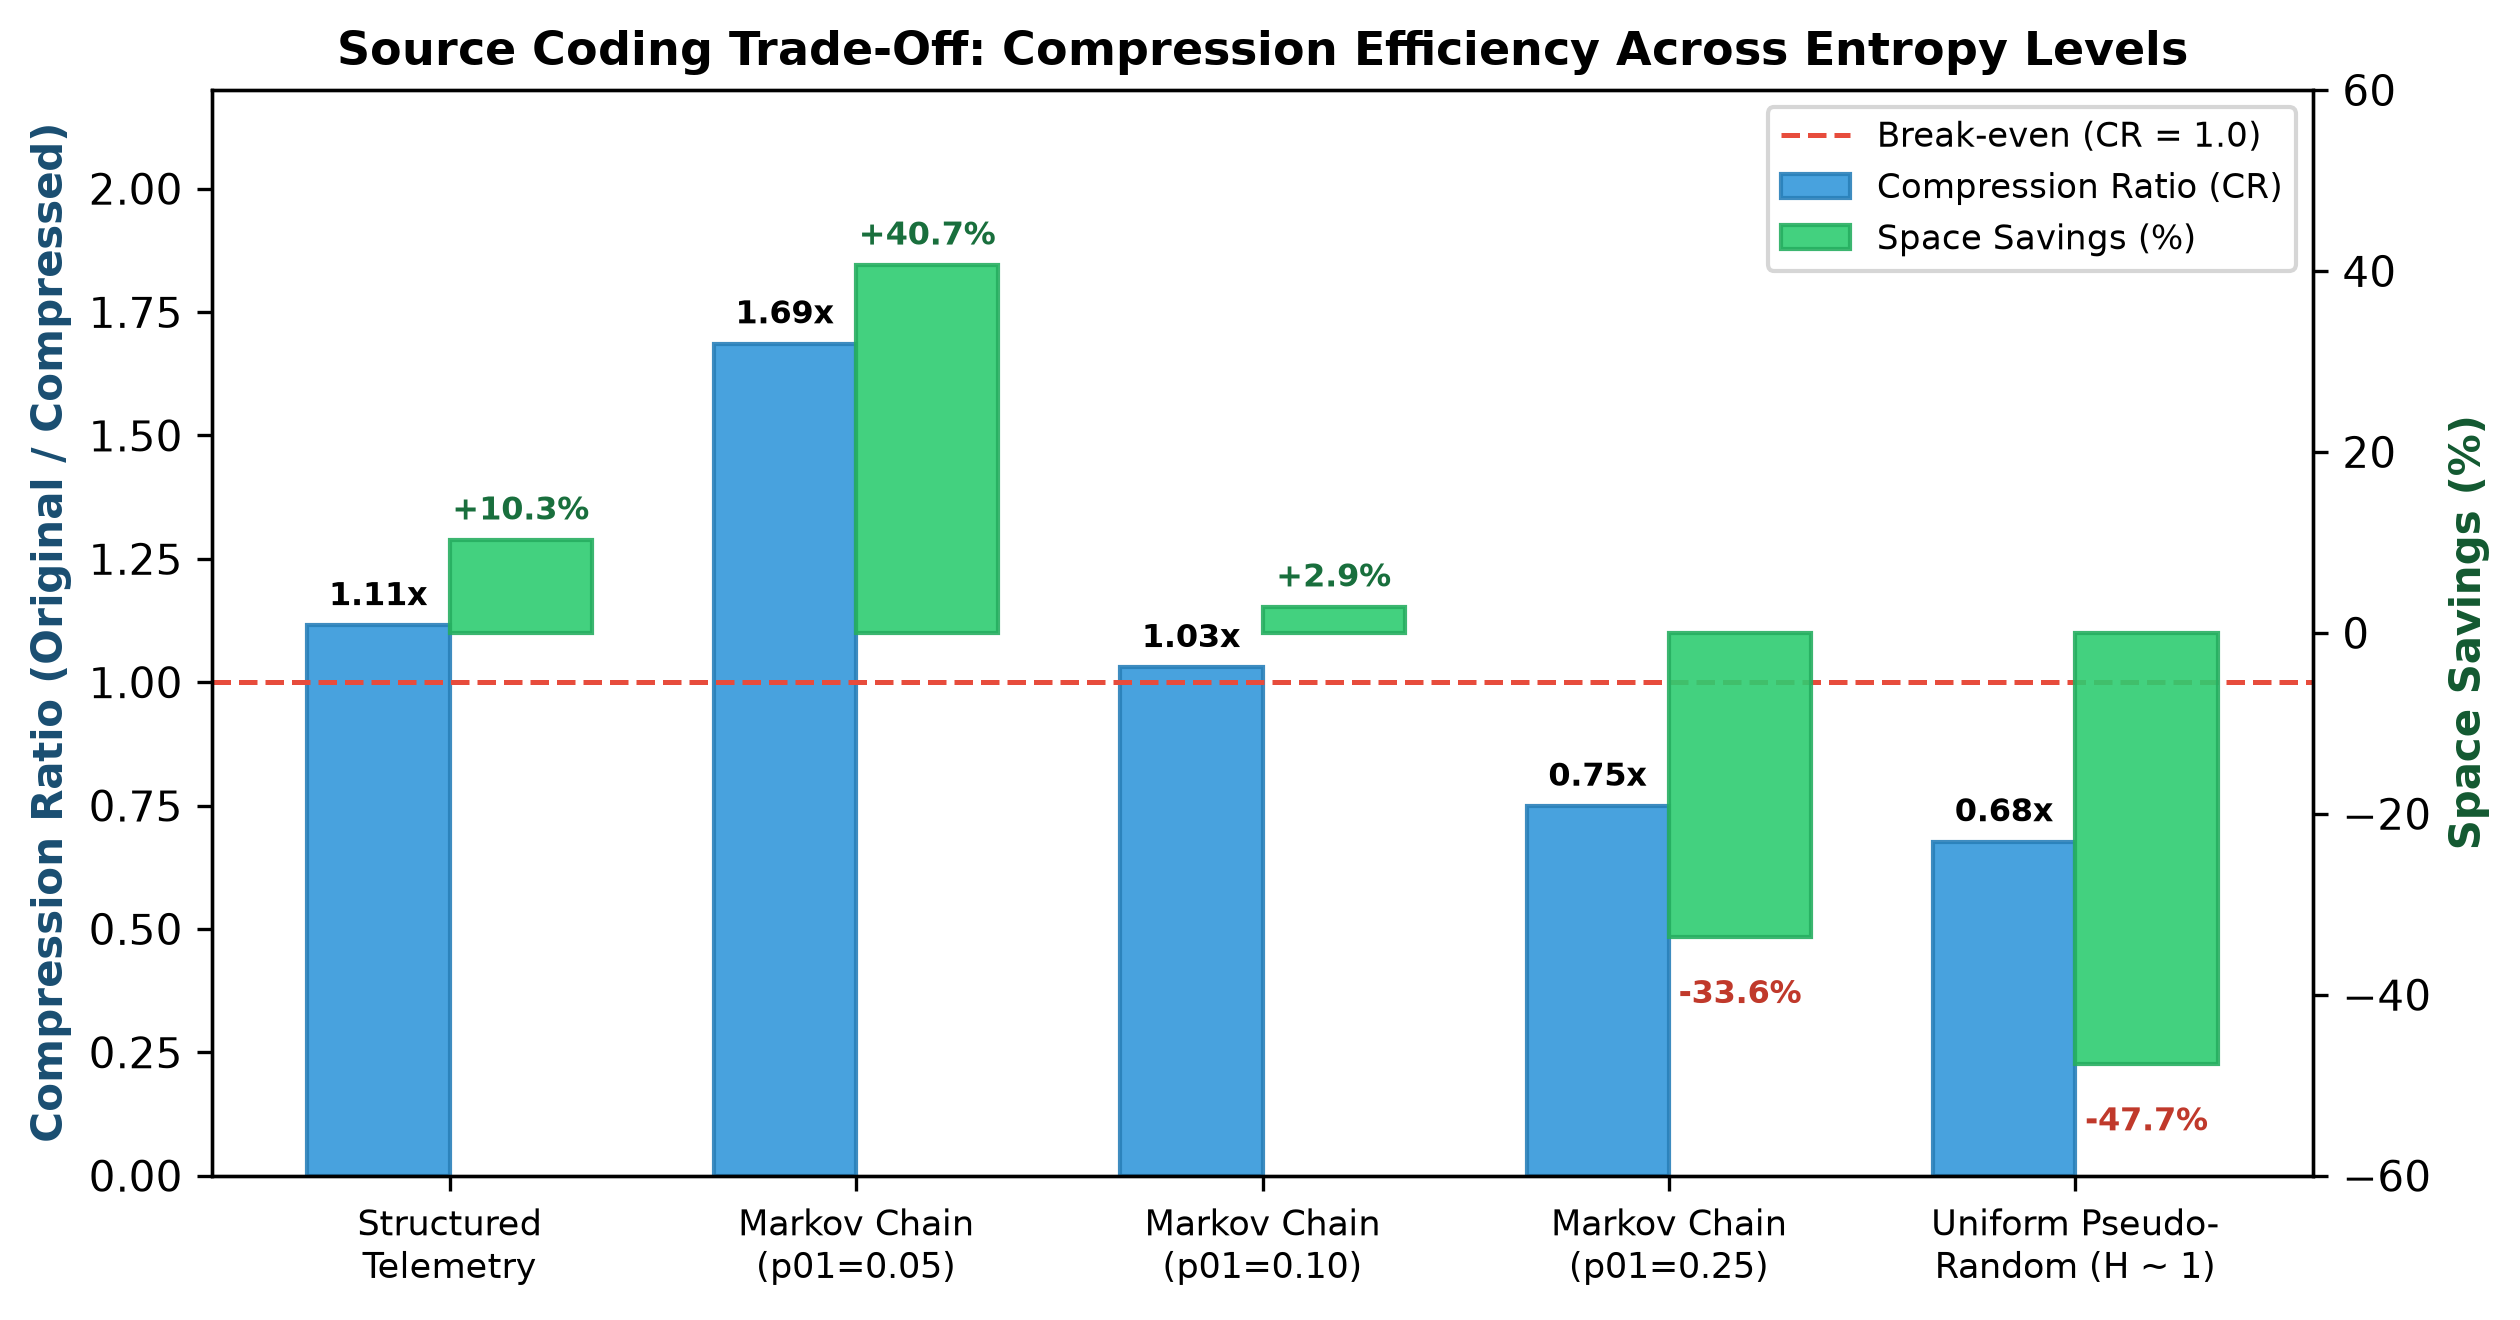
\includegraphics[width=\columnwidth]{figures/fig5_source_coding_entropy.png}
\caption{Source coding trade-off: empirical Shannon entropy versus compression ratio and percentage space savings across diverse information source topologies.}
\label{fig:source_comp}
\end{figure}

\begin{table}[htbp]
\caption{Source Compression Study Across Diverse Information Topologies}
\label{tab:source_results}
\centering
\scriptsize
\begin{tabular}{lccccc}
\toprule
Source Topology & $H(X)$ & Raw & Comp. & CR & Savings \\
& (bits) & (bits) & (bits) & & (\%) \\
\midrule
Structured Telemetry & 4.7612 & 5216 & 4680 & 1.115 & +10.28\% \\
Markov ($p_{01}=0.05, p_{10}=0.05$) & 0.9996 & 8192 & 4860 & 1.686 & +40.67\% \\
Markov ($p_{01}=0.10, p_{10}=0.20$) & 0.9228 & 8192 & 7956 & 1.030 & +2.88\% \\
Markov ($p_{01}=0.25, p_{10}=0.25$) & 0.9996 & 8192 & 10944 & 0.749 & -33.59\% \\
Uniform Pseudo-Random & 1.0000 & 8192 & 12096 & 0.677 & -47.66\% \\
\bottomrule
\end{tabular}
\end{table}

\begin{figure}[t]
\centering
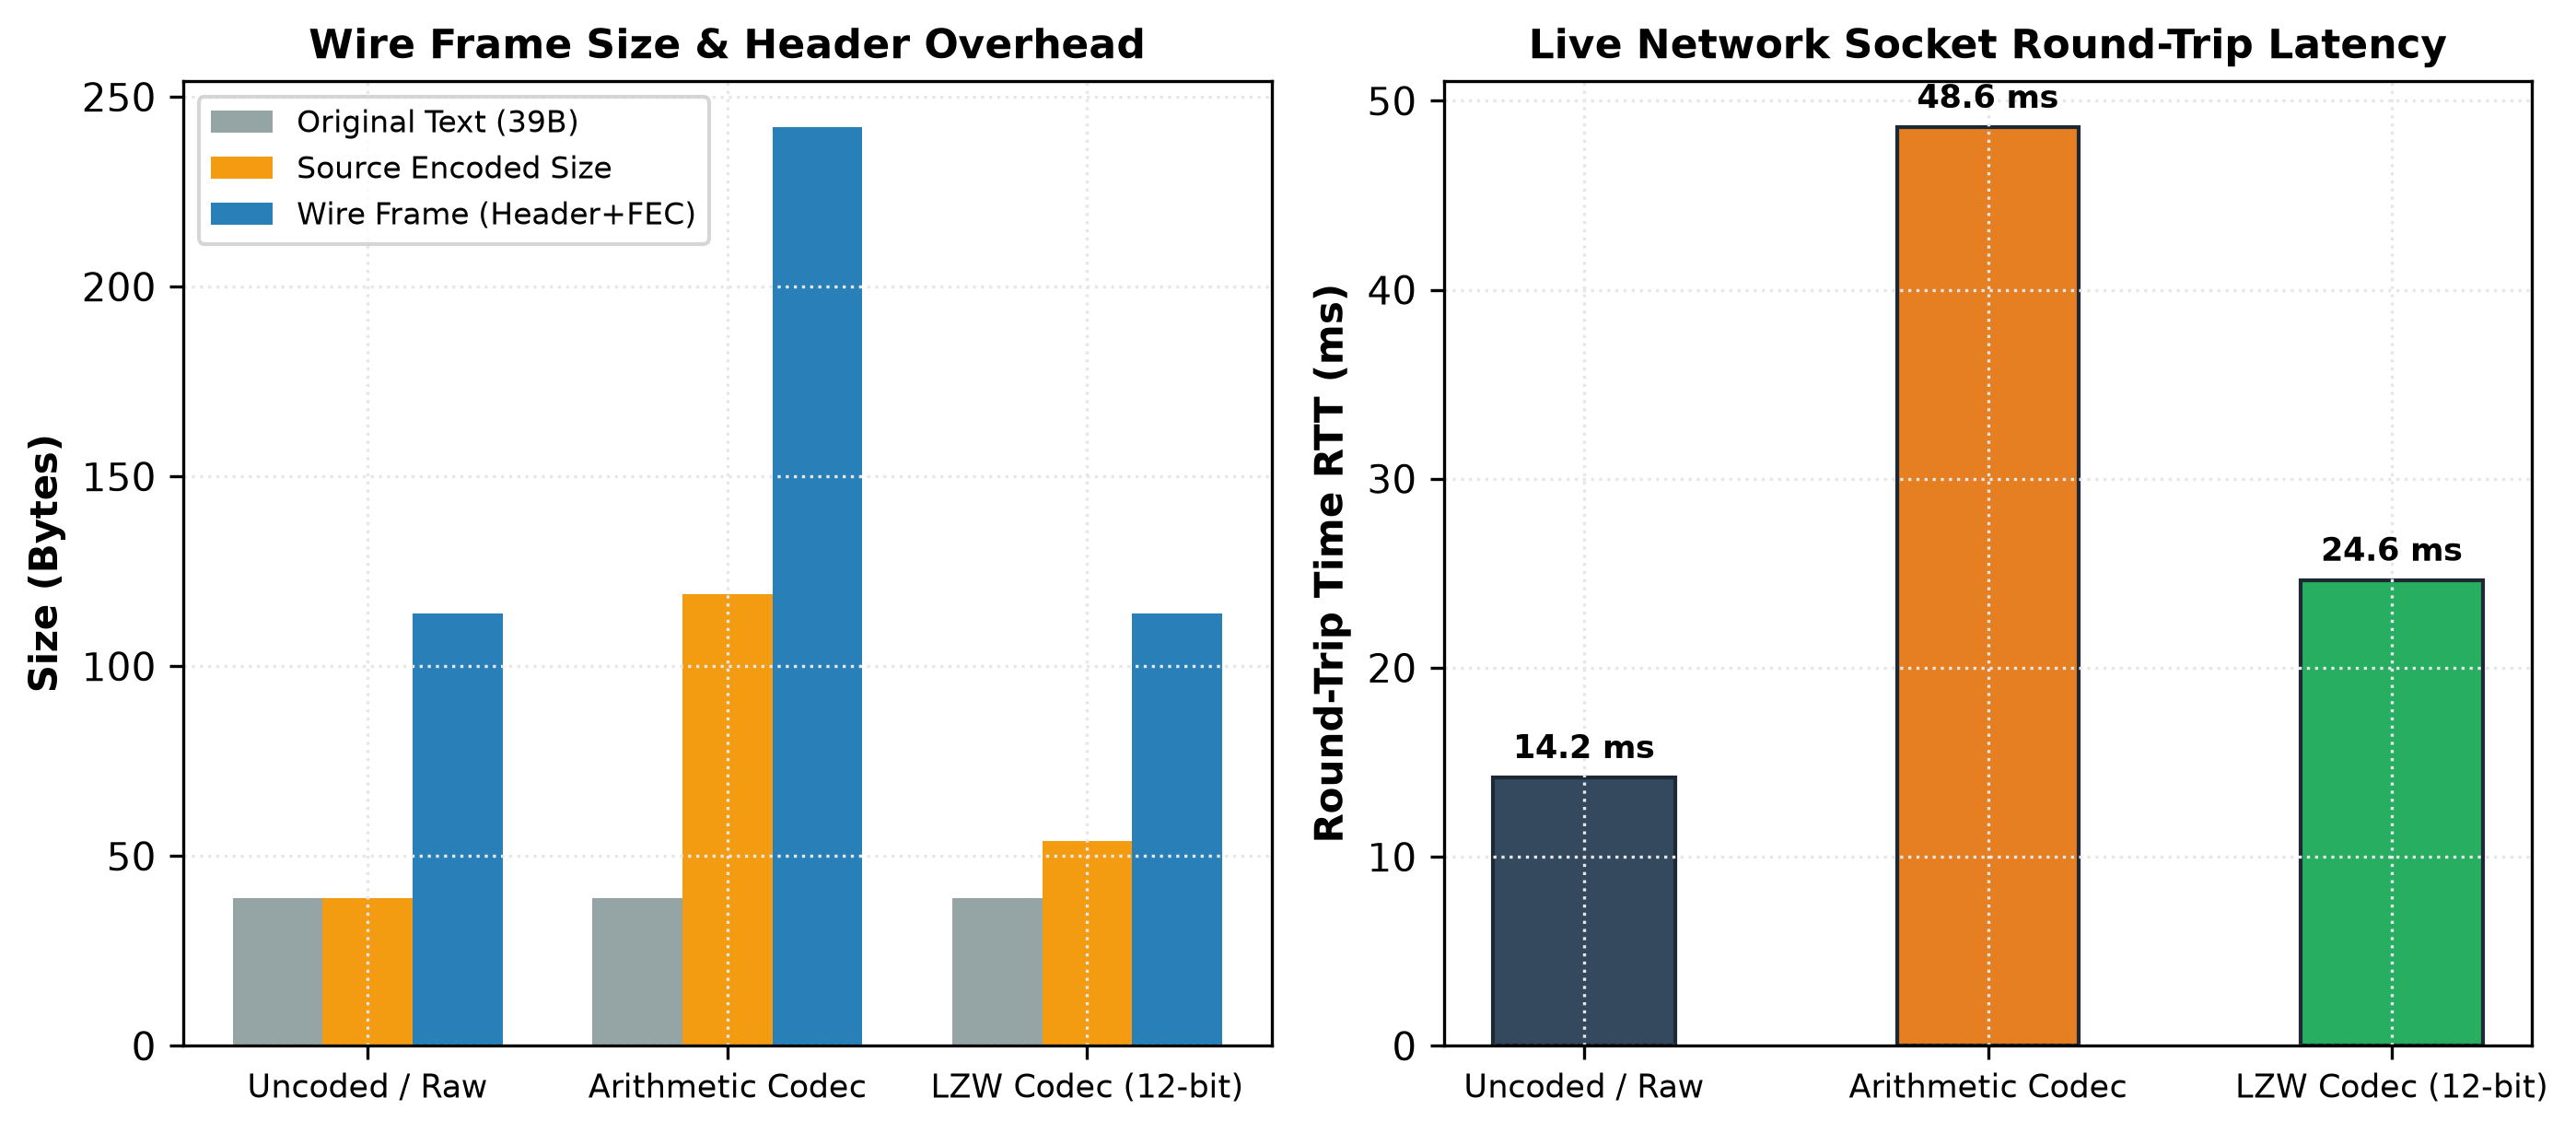
\includegraphics[width=\columnwidth]{figures/fig6_socket_latency_overhead.png}
\caption{Live wireless network socket benchmark (Mode A): transmitted frame size breakdown (left) and round-trip ACK latency (right) for raw text, Arithmetic coding, and LZW coding.}
\label{fig:socket_bench}
\end{figure}

\subsection{Live Wireless Network Socket Transfer (Mode A)}
Table~\ref{tab:socket_results} and Fig.~\ref{fig:socket_bench} report measured performance over TCP sockets transmitting \texttt{"Hello, this is my wireless ITC project!"} ($39$ bytes). All frames were verified with valid CRC32 checksums and received sequence-confirmed acknowledgments. Round-trip latency was $14.20$~ms (raw text), $24.64$~ms (LZW), and $48.60$~ms (Arithmetic), reflecting byte serialization and LDPC parity matrix multiplications.

\begin{table}[htbp]
\caption{Live Wireless Socket Transmission Metrics (Mode A)}
\label{tab:socket_results}
\centering
\scriptsize
\begin{tabular}{lccccc}
\toprule
Codec Mode & Orig. Size & Src. Size & Frame Size & Latency & Checksum \\
& (Bytes) & (Bytes) & (Bytes) & (ms) & Fidelity \\
\midrule
Raw Text & 39 & 39 & 114 & 14.20 & CRC32 OK / 100\% \\
Arithmetic & 39 & 119 & 242 & 48.60 & CRC32 OK / 100\% \\
LZW (12-bit) & 39 & 54 & 114 & 24.64 & CRC32 OK / 100\% \\
\bottomrule
\end{tabular}
\end{table}

\subsection{Comparison of Supported Coding Configurations}
Table~\ref{tab:codecs_comp} provides a comprehensive comparison of all coding schemes supported by the codebase.

\begin{table}[htbp]
\caption{Supported Channel Coding Configurations Benchmark}
\label{tab:codecs_comp}
\centering
\scriptsize
\begin{tabular}{lcccc}
\toprule
\textbf{Metric} & \textbf{Hamming (7,4)} & \textbf{Polar (64,32)} & \textbf{LDPC Min-Sum} & \textbf{LDPC Sum-Prod} \\
\midrule
Blocklength ($N, K$) & $(7, 4)$ & $(64, 32)$ & $(64, 32)$ & $(64, 32)$ \\
Code Rate ($R$) & $0.571$ & $0.500$ & $0.500$ & $0.500$ \\
Decoding Paradigm & Syndrome Table & Successive Canc. & Min-Sum BP & Sum-Product BP \\
Complexity & $\mathcal{O}(1)$ lookup & $\mathcal{O}(N \log N)$ & $\mathcal{O}(I \cdot d_v N)$ & $\mathcal{O}(I \cdot d_v N)$ transcendental \\
BER at $4.0$~dB & $1.68 \times 10^{-2}$ & $2.38 \times 10^{-3}$ & $2.85 \times 10^{-3}$ & $\mathbf{1.99 \times 10^{-3}}$ \\
Zero-Error SNR & $\ge 8.0$~dB & $\ge 5.0$~dB & $\ge 7.0$~dB & $\ge 7.0$~dB \\
Application & Control/Header & 5G Control & Low-power ASIC & High-performance Data \\
\bottomrule
\end{tabular}
\end{table}

\subsection{Coupling of Channel Errors and Source Decompression}
When source coding is applied, uncorrected channel errors cause catastrophic desynchronization. At $E_b/N_0 = 4.0$~dB, two residual block errors corrupted the compressed bitstream, causing the Arithmetic decompressor to raise a \texttt{MalformedStreamException} and fail message recovery. Only at $E_b/N_0 \ge 7.0$~dB, where LDPC eliminated all errors, was $100\%$ exact message reconstruction achieved.

\section{Discussion and Limitations}
Several engineering considerations and constraints must be noted:
\begin{enumerate}
    \item \textbf{Simulated AWGN vs. Real Radio Propagation:} The physical simulation uses additive white Gaussian noise. Physical wireless environments (e.g., Wi-Fi IEEE 802.11) encounter multipath scattering, Rayleigh/Rician fading, Doppler shifts, and hardware frequency offsets \cite{tse2005}, which are not captured in software baseband simulation.
    \item \textbf{TCP ARQ Masking:} Sockets in Mode A operate over TCP/IP, where packet retransmission and congestion control mask underlying physical layer bit errors. This provides reliable application transport but prevents observation of raw radio packet loss.
    \item \textbf{Short LDPC Blocklength ($N=64$):} While computationally lightweight, short codes exhibit wider waterfall regions and higher error floors than large standardized codes (such as IEEE 802.3an $N=2048$ or 5G NR $N=1024$).
    \item \textbf{Sample Size Constraints:} Evaluating extreme error floors ($\text{BER} \le 10^{-8}$) requires transmitting over $10^9$ bits, exceeding CPU runtime budgets for interactive software simulation.
\end{enumerate}

\section{Conclusion and Future Work}
This paper presented the design, implementation, and empirical verification of an end-to-end digital communication simulation system. By integrating finite-precision Arithmetic coding, adaptive LZW compression, systematic rate-$1/2$ LDPC $(64, 32)$ coding with log-domain Belief Propagation, and a 36-byte versioned binary frame protocol with CRC32 integrity verification, the system successfully bridges theoretical information theory and real-world networking. Empirical evaluations demonstrated that the LDPC decoder achieves a $43.3\times$ error suppression gain at $E_b/N_0 = 4.0$~dB and delivers error-free transmission ($\text{BER} = 0.0000$) with $100\%$ exact text reconstruction at $E_b/N_0 \ge 7.0$~dB.

Future extensions of this work include:
\begin{enumerate}
    \item Integrating higher-order digital modulations, such as Quadrature Phase Shift Keying (QPSK) and 16/64-QAM with Orthogonal Frequency Division Multiplexing (OFDM).
    \item Scaling the LDPC codec to standardized quasi-cyclic parity-check matrices ($N \ge 1024$) utilizing GPU-accelerated Belief Propagation.
    \item Interfacing the physical layer simulation with Software-Defined Radio (SDR) hardware (e.g., RTL-SDR, HackRF, or USRP) to conduct over-the-air radio frequency transmissions.
\end{enumerate}

\bibliographystyle{IEEEtran}
\bibliography{references}

\end{document}
